%Typeset using XeLaTeX

\documentclass[10pt,a4paper,twoside]{book}
\usepackage{amsmath,amssymb,amsthm}
\usepackage{phonetic}
\usepackage{fancyhdr}
\usepackage[pass]{geometry}
\usepackage{fontspec}
\usepackage{xunicode}
\usepackage{xltxtra}
\usepackage{fancyhdr}
\usepackage{fontspec}
\usepackage[toc,page]{appendix}
%\usepackage{polyglossia}
\usepackage{enumitem}
\usepackage{amsfonts}
\usepackage{bm}
\usepackage{subcaption}
\usepackage{graphicx}
\usepackage{caption}
\usepackage{graphbox}
\usepackage{tabularx}
\usepackage{arydshln}
\usepackage{textcomp}
\usepackage{mathrsfs}
\usepackage{soul}
\usepackage{hyperref}
\usepackage[dvipsnames]{xcolor}
\usepackage{verbatim}
\usepackage{lmodern}
\usepackage{algorithm,algpseudocode}
\usepackage{mathtools}
\usepackage{fancybox,framed}
\usepackage{multicol}
\usepackage{tcolorbox}
\usepackage{multirow}
\usepackage{listings}
%\usepackage{xgreek}
\setmainfont[Ligatures=TeX]{Linux Libertine O}
%\setmainfont[Mapping=TeX-text]{Times New Roman}
\usepackage{color}
\usepackage[Glenn]{fncychap}
\ChNameVar{\bfseries\Large}
\usepackage[normalem]{ulem}
\usepackage[colorinlistoftodos]{todonotes}

%-------------------------------------------------
% BIB TEX
%-------------------------------------------------
\usepackage[style=alphabetic,citestyle=alphabetic,giveninits=true,doi=false,isbn=false,url=false,date=year,maxnames=3]{biblatex}
\renewbibmacro{in:}{}
\AtBeginBibliography{\renewcommand*{\mkbibnamefamily}[1]{\MakeUppercase{#1}}}
\addbibresource{thesis_refs.bib}
\renewcommand\multicitedelim{\addcomma\space}

%\usepackage{hyperref}
\hypersetup{
    linktocpage = true,
    colorlinks = true,
    citecolor = {BrickRed},
    linkcolor = {BrickRed},
    %linkcolor = {NavyBlue},
    urlcolor = {cyan}
}

\pagestyle{fancy}
\fancyhf{}%clear all headers and footers
\fancyhead[LO]{\slshape \leftmark}
\fancyhead[RE]{\slshape \rightmark}
\fancyhead[LE, RO]{\thepage}
\fancyfoot[LO,RE]{\tiny{\it}}

\setlength{\parindent}{1em}
\emergencystretch=1em
%-------------------------------------------------
% NEW COMMANDS AND MATH OPERATORS
%-------------------------------------------------
\renewcommand\qedsymbol{$\blacksquare$}

\newcommand{\mbf}[1]{\mbox{\boldmath$\rm{#1}$}}
\newcommand{\bx}{\mbf{x}}
\newcommand{\by}{\mbf{y}}
\newcommand{\bz}{\mbf{z}}
\newcommand{\bw}{\mbf{w}}
\newcommand{\mbfb}[1]{\mbox{\boldmath$\bar{\rm{#1}}$}}

\newcommand{\cauchy}{\mathcal{D}_C}
\newcommand{\ha}{\frac{1}{2}}
\newcommand{\real}[1]{\mathbb{R}^{#1}}
\newcommand{\binar}[1]{\{0,1\}^{#1}}
\newcommand{\bd}{\{0,1\}^d}
\newcommand{\rd}{\mathbb{R}^{d}}
\newcommand{\rk}{\mathbb{R}^{k}}
\newcommand{\dx}{\,\mathrm{d} x}
\newcommand{\du}{\,\mathrm{d} u}
\newcommand{\ex}{{\rm e}}
\newcommand{\eps}{\varepsilon}
\newcommand{\net}{\mathcal{N}}
\newcommand{\grid}{\mathcal{G}}
\newcommand{\cell}{\mathcal{C}}

\newcommand{\norm}[1]{\left \rVert {#1} \right \rVert}
\newcommand{\abs}[1]{\left \rvert {#1} \right \rvert}

\DeclareMathOperator*{\argmin}{arg\,min}
\DeclareMathOperator*{\argmax}{arg\,max}
\DeclareMathOperator*{\prob}{\mathbf{Pr}}
\DeclareMathOperator*{\var}{\mathbf{Var}}
\DeclareMathOperator*{\EE}{\mathbb{E}}

%-------------------------------------------------
% THEOREMS
%-------------------------------------------------

\theoremstyle{definition}
\newtheorem{definition}{Definition}[chapter]
\newtheorem*{definition*}{Definition}
\newtheorem{theorem}[definition]{Theorem}
\newtheorem{lemma}[definition]{Lemma}
\newtheorem{corollary}[definition]{Corollary}
\theoremstyle{remark}
\newtheorem{remark}{Remark}
\newtheorem{example}[definition]{Example}
\newtheorem{claim}[definition]{Claim}
\newtheorem{fact}[definition]{Fact}

\newtheorem*{claim*}{Claim}


%-------------------------------------------------
% TITLE PAGE
%-------------------------------------------------

\renewcommand{\maketitle}{
\begin{titlepage}
\newgeometry{left=4cm, top=2.3cm, bottom=2.3cm}
\hbox{\mbox{\hspace{-1.3cm}}
\vrule depth 0.98\textheight
\mbox{\hspace{1cm}}
\vtop{
\vspace{2cm}
\begin{flushleft}
\huge{\bf Dimensionality reduction for approximate near neighbor search in the Manhattan metric\\}
\vskip3cm
\Large  Vasileios Margonis\\
R.N. A0005\\
\vskip3cm
\begin{minipage}{7.5cm}
\begin{flushleft}
\normalsize {\it {\bf Examination committee:}\\
Ioannis Emiris, Department of Informatics \& Telecommunications, NKUA.\\
Aris Pagourtzis, School of Electrical \& Computer Engineering, NTUA. \\
Dimitris Fotakis, School of Electrical \& Computer Engineering, NTUA.}
\end{flushleft}
\end{minipage}
\hskip0.5cm
\begin{minipage}{6cm}
\begin{flushleft}
\normalsize {\it {\bf Supervisor:}\\
Ioannis Emiris, Professor, \\ Department of Informatics \& Telecommunications,\\
NKUA.\\
}
\end{flushleft}
\end{minipage}
\end{flushleft}
\vskip5.5cm
\hskip4.5cm
\begin{minipage}{5cm}
\begin{center}
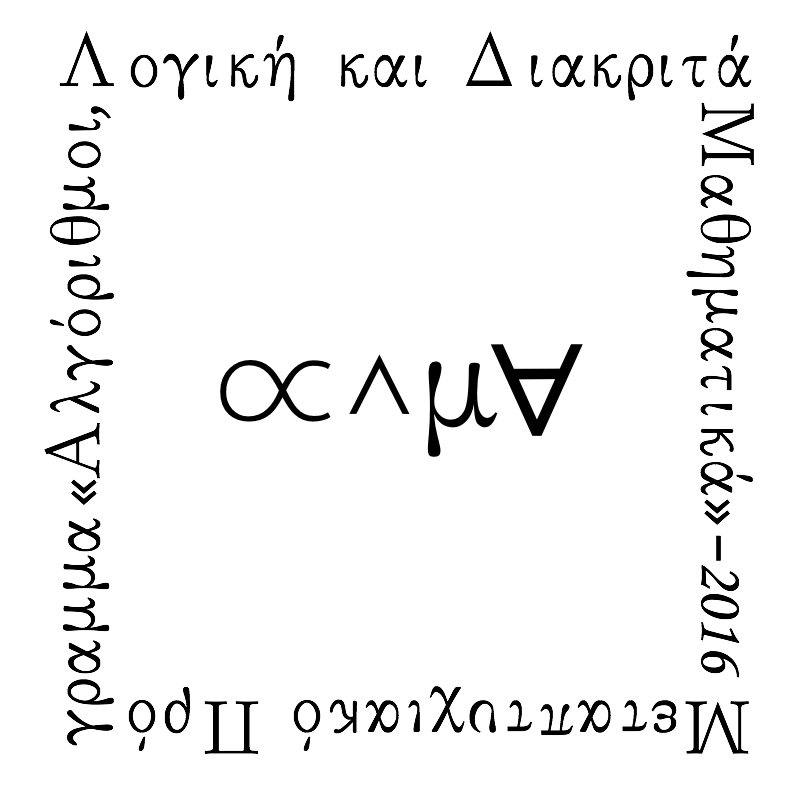
\includegraphics[width=0.8\textwidth]{figures/alma.png}
\end{center}
\end{minipage}
\vfill
\hfill April, 2019
}
}
\end{titlepage}
}

%-------------------------------------------------
% BEGIN DOCUMENT
%-------------------------------------------------

\begin{document}

\maketitle
\clearpage

\thispagestyle{empty}
\null
\clearpage

\thispagestyle{empty}
\newgeometry{margin=3.5cm, top=5cm}

{\large
\begin{center}

\includegraphics[width=0.25\textwidth]{figures/uoalogo.jpg} \\ \vskip0.1cm
Η παρούσα Διπλωματική Εργασία\\ \vskip0.1cm
εκπονήθηκε στα πλαίσια των σπουδών\\ \vskip0.1cm
για την απόκτηση του\\ \vskip0.1cm
{\bf Μεταπτυχιακού Διπλώματος Ειδίκευσης}\\ \vskip0.1cm
{\bf «Αλγόριθμοι, Λογική και Διακριτά Μαθηματικά»}\\ \vskip0.1cm
που απονέμει το \\ \vskip0.1cm
{\bf Τμήμα Πληροφορικής και Τηλεπικοινωνιών\\ \vskip0.1cm
του \\ \vskip0.1cm
Εθνικού και Καποδιστριακού Πανεπιστημίου Αθηνών}\\

\vskip1.3cm

Εγκρίθηκε την 11η Απριλίου 2019 από Εξεταστική Επιτροπή \\ 
\vskip0.1cm
αποτελούμενη από τους:
\end{center}

\vskip0.3cm
\renewcommand{\arraystretch}{3.6}

\newcolumntype{A}[1]{>{\hsize=#1\hsize\raggedright\arraybackslash}X}
\newcolumntype{K}[1]{>{\hsize=#1\hsize\centering\arraybackslash}X}

\begin{table}[htbp]
\centering
\begin{tabularx}{\textwidth}{K{0.5}K{0.5}}
\uline{\bf \large Ονοματεπώνυμο} & \uline{\bf \large Βαθμίδα}\\
1. \large Ιωάννης Εμίρης & \large Καθηγητής\\
2. \large Άρης Παγουρτζής & \large Αναπλ. καθηγητής \\
3. \large Δημήτρης Φωτάκης & \large Αναπλ. καθηγητής \\
\end{tabularx}
\end{table}
\iffalse
\begin{table}[htbp]
\centering
\begin{tabularx}{\textwidth}{K{0.4}K{0.4}K{0.2}}
\uline{\bf \large Ονοματεπώνυμο} & \uline{\bf \large Βαθμίδα} & \uline{\bf \large Υπογραφή}\\
1. \large Ιωάννης Εμίρης & \large Καθηγητής & \dotfill \\
2. \large Άρης Παγουρτζής & \large Αναπλ. καθηγητής & \dotfill \\
3. \large Δημήτρης Φωτάκης & \large Αναπλ. καθηγητής & \dotfill \\
\end{tabularx}
\end{table}
\fi
}


\clearpage

\thispagestyle{empty}
\null 
\clearpage

\restoregeometry

\thispagestyle{empty}
\pagenumbering{gobble}
\chapter*{Abstract}
The approximate nearest neighbor problem is one of the fundamental problems in computational geometry and has received much attention during the past decades. Efficient and practical algorithms are known for data sets of low dimension. However, modern, high-dimensional data cannot be handled by these algorithms, because of the so called ``curse of dimensionality". A new theory for approximate nearest neighbors in high dimensions emerged with an influential paper by Indyk and Motwani, in 1998, yielding algorithms that depend polynomially on the dimension. 

Nevertheless, is has been realized that designing efficient ANN data structures is closely related with dimension-reducing embeddings. One popular dimension reduction technique is randomized projections. Starting with the celebrated Johnson-Lindenstrauss Lemma, such projections have been studied in depth for the Euclidean $(\ell_2)$ metric and, much less, for the Manhattan $(\ell_1)$ metric. In 2007, Indyk and Naor, in the context of approximate nearest neighbors, introduced the notion of nearest neighbor-preserving embeddings. These are randomized embeddings between two metric spaces with guaranteed bounded distortion only for the distances between a query point and a point set. Such embeddings are known to exist for both $\ell_2$ and $\ell_1$ metrics, as well as for doubling subsets of $\ell_2$.

In this thesis, we consider the approximate nearest neighbor problem in doubling subsets of $\ell_1$. We exploit the decision-with-witness version, called approximate \textit{near} neighbor, which incurs a roughly logarithmic overhead, and we propose a dimension reducing, \textit{near} neighbor-preserving embedding for doubling subsets of $\ell_1$. Our approach is to represent the point set with a carefully chosen covering set, and then apply a random linear projection to that covering set, using a matrix of Cauchy random variables. We study two cases of covering sets: approximate nets and randomly shifted grids, and we discuss the differences between them in terms of computing time, target dimension, as well as their algorithmic implications.

\vfill
\paragraph{Keywords and phrases} Approximate nearest neighbor, dimensionality reduction, Manhattan metric, randomized embedding

\clearpage

\thispagestyle{empty}
\null 
\clearpage

\thispagestyle{empty}
\pagenumbering{gobble}
\chapter*{Σύνοψη}
%\emergencystretch=2em
Οι τυχαίες προβολές αποτελούν μια απο τις πιο διαδεδομένες μεθόδους για το χειρισμό δεδομένων μεγάλης διάστασης. Ξεκινώντας από το περίφημο Johnson-Lindenstrauss Lemma, τέτοιου είδους προβολές έχουν μελετηθεί αρκετά για την Ευκλείδια $(\ell_2)$ μετρική, και πολύ λιγότερο για τη μετρική Μανχάταν $(\ell_1)$. Σε αυτή την εργασία εστιάζουμε στο πρόβλημα του προσεγγιστικού κοντινότερου γείτονα στη μετρική Μανχάταν, εκμεταλλεύοντας την αποφαντική εκδοχή του προβλήματος, που λέγεται προσεγγιστικός \textit{κοντινός} γείτονας και επιβάλει ένα (περίπου) λογαριθμικό κόστος.

Το 2007, οι Indyk και Naor εισήγαγαν την έννοια των εμβυθίσεων που διατηρούν τον κοντινότερο γείτονα (nearest neighbor-preserving embeddings). Οι εμβυθίσεις αυτές είναι τυχαιοκρατικές και εγγυόνται για την αλλοίωση μόνο $n$ αποστάσεων (μεταξύ ενός σημείου-query και $n$ σημείων), αντί για όλα τις δυνατές $O(n^2)$. Τέτοιου είδους εμβυθίσεις υπάρχουν για τις μετρικές $\ell_2$ και $\ell_1$, καθώς και για διπλασιάζοντα (doubling) υποσύνολα της $\ell_2$.

Σε αυτή την εργασία παρουσιάζουμε μια συνάρτηση εμβύθισης για την μείωση διάστασης, η οποία διατηρεί τον \textit{κοντινό} γείτονα (\textit{near} neighbor-preserving) για διπλασιάζοντα υποσύνολα της $\ell_1$. Η τεχνική που εφαρμόζουμε είναι να προβάλουμε τυχαία όχι τα ίδια τα σημεία, αλλά ένα σύνολο αντιπροσώπων τους. Μελετούμε δύο είδη αντιπροσώπων, τα approximate nets και τα randomly shifted grids, και τα συγκρίνουμε ως προς την νέα διάσταση και το χρόνο υπολογισμού της συνάρτησης εμβύθισης.

\clearpage

\thispagestyle{empty}
\null 
\clearpage

\chapter*{Acknowledgements}

First and foremost I would like to thank my supervisor, Prof. Ioannis Emiris, for his guidance, support, and excellent advice.

Of course, I want to express my deep gratitude to Ioannis Psarros, for our productive and stimulating cooperation throughout the whole process of researching this thesis.

I also want to thank Prof. Aris Pagourtzis and Prof. Dimitris Fotakis, for their participation in the examination committee.

Finally, I want to thank my family and my friends, for their unconditional and continued support.

\clearpage

\thispagestyle{empty}
\null 
\clearpage


\clearpage
\thispagestyle{empty}

\pagestyle{fancy}

\pagenumbering{roman}
\tableofcontents
\clearpage

\thispagestyle{empty}
\null 
\clearpage

\pagenumbering{arabic}

%-------------------------------------------------------------------------------
\chapter{Introduction}
%-------------------------------------------------------------------------------

The \textit{nearest neighbor} problem is defined as follows: Given a set $P$ of $n$ points in a metric space $(X,d_X)$, build a data structure that, given any query point $q \in X$, returns its ``nearest neighbor" $\argmin_{p \in P} d_X(q,p)$. A particularly interesting case is that of geometric spaces, where $X = \rd$ and $d_X$ is induced by some norm. The most popular metrics are the Euclidean $(\ell_2)$ and the Manhattan $(\ell_1)$. This problem, and its approximate versions, are some of the central problems in computational geometry, and have a wide range of applications in machine learning, computer vision, data compression and other fields \cite{SDI06, Dub10, MO15}. 

A common relaxation is the $c$-\textit{approximate nearest neighbor} problem, where the data structure is allowed to report any $p' \in P$ within distance $c \cdot \min_{p \in P} d_X(q,p)$; for some approximation factor $c \geq 1$. By known reductions \cite{IM98}, one may focus on the \textit{decision-with witness} version, which incurs a polylogarithmic overhead:
\begin{definition}[Approximate Near Neighbor]
Let $(X,d_X)$ be a metric space. Given $P \subseteq X$ and reals $R>0$, $c \geq 1$, build a data structure $\mathcal{S}$ that, given a query point $q \in X$, performs as follows:
\begin{itemize}
\itemsep0em
    \item If the nearest neighbor of $q$ lies in distance at most $R$, then $\mathcal{S}$ is allowed to report any point $p^* \in P$ such that $d_X(q,p^*) \leq cR$.
    \item If all points lie at distance more than $cR$ from $q$, then  $\mathcal{S}$ should return $\bot$.
\end{itemize}
$\mathcal{S}$ is allowed to return either a point at distance $\leq cR$ or $\bot$. 
\end{definition}

From now on, we shall refer to this problem as $c$-ANN, or simply ANN. Typically, the performance of an ANN data structure is measured by three quantities: 1) \textit{preprocessing} -- time to build it, 2) \textit{space} -- amount of memory it occupies and, 3) \textit{query time} -- time it takes to return an answer, given a query.

Depending on the relation between the dimension $d$ and the number of data points $n$, two main regimes have emerged: low- and high-dimensional. The low-dimensional regime corresponds to $ d=o(\log{n})$; (hence algorithms can afford to be exponential in the dimension) and the high-dimensional regime corresponds to $d = \omega(\log n)$.

%-------------------------------------------------------------------------------
\section{Previous work} \label{section:prev}
%-------------------------------------------------------------------------------

In the low-dimensional regime, efficient $(1{+}\eps)$-ANN algorithms are known for the Euclidean space. One notable data-structure is the Balanced Box-Decomposition (BBD) tree, introduced in \cite{AMNSW98}. BBD trees achieve query time $O(c \log n$), for $c \leq d/2 \lceil 1+6d/ \eps \rceil^d$, space $O(dn)$ and preprocessing time $O(dn \log n)$, and can also be used to retrieve the $k \leq 1 $ approximate nearest neighbors, with an extra $O(d \log n)$ cost per neighbor. They are very practical as well.

Another popular data structure for $\ell_2$, is the Approximate Voronoi Diagrams (AVD) \cite{AMM09}, where a tradeoff is established between space requirement and query time. More specifically, for a tradeoff parameter $2< \gamma < 1/ \eps$, the query time is $O(\log (n \gamma) + 1/(\eps \gamma)^{\frac{d-1}{2}})$ and space is $O(n \gamma^{d-1} \log (1/ \eps))$. This data structure maintains a hierarchical subdivision of space into cells, each storing a number of representatives, such that for any query lying in some cell, at least one of the representatives is an approximate nearest neighbor. Further improvements to the space-time trade offs for ANN are obtained in \cite{AdFM18}.

The bucketing method of \cite{HIM12} admits a data structure that supports fast queries for any $\ell_p$, $p \in [1,2]$, with space and preprocessing time $O(1/ \eps)^d \times O(n)$ and query time $O(d)$. This is done by imposing a grid on the data set, and then storing grid points which lie close to data points in a hash function. 

All the aforementioned methods however, are based on discretization of the input space, and therefore depend exponentially in $d$, making them unfit for high-dimensional data. 

An important method conceived for high dimensional data is Locality-Sensitive Hashing (LSH), introduced in \cite{IM98}. It relies on the existence of locality sensitive hash functions for the input space, which are more likely to map similar objects to the same bucket \footnote{See also Section \ref{section:lsh}}. In general, LSH requires roughly $O(dn^{1+\rho})$ space and $O(dn^{\rho})$ query time for some parameter $\rho \in (0,1)$. Upper bounds of $\rho$ have been established for $c$-ANN in $\ell_2$ and $\ell_1$ norms; $\rho = 1/c^2 + o(1)$ for $\ell_2$ and $\rho = 1/c + o(1)$ for $\ell_1$ \cite{AI08, IM98}, as well as matching lower bounds \cite{MNP07, OWZ14}. LSH schemes based on $p$-stable distributions also exist for $\ell_p, p \in (0,2]$ \cite{DIIM04}, with $\rho \leq (1 {+} \gamma) \cdot \max{(1/c^p, 1/c)}$, for any $\gamma>0$.

Better bounds on $\rho$ can be obtained via \textit{data-dependent LSH}: random space partitions which depend on the data set. Namely, we get $\rho= 1/(2c-1) + o(1)$ for $\ell_1$ and $\rho= 1/(2c^2-1) + o(1)$ for $\ell_2$ \cite{AINR14, AR15}. These bounds are also known to be tight in the data-dependent LSH framework \cite{AR16}. Moreover, upper and lower bounds for time-space tradeoffs have also been studied for both data-dependent and data-independent LSH \cite{ALRW17}.

Spaces which are considered to be harder in this context, like $\ell_{\infty}$, can also be treated \cite{Ind01, Chan17}, and are very interesting since they can be used as host spaces for various symmetric norms \cite{ANNRW17} (e.g., top-$k$ and Orlicz norms)

It has become apparent that designing efficient ANN algorithms, at least for high-dimensional data, is closely related to the task of designing \textit{low-distortion} embeddings.

\begin{definition} \label{bilips}
A \textit{bi-Lipschitz embedding} between two metric spaces $(X,d_X)$ and $(Y,d_{Y})$ is a mapping $f: X \rightarrow Y $ such that for some scaling factor $C>1$, and \textit{distortion} $D \geq 1$, for every $p, q \in X$ 
\begin{equation*}
    C \cdot d_X(p,q) \leq d_{Y}(f(p),f(q)) \leq D \cdot C \cdot d_X(p,q).
\end{equation*}
\end{definition}

Of particular importance, are low-distortion embeddings that map $\rd$ to $\mathbb{R}^k$, where $k$ is much smaller than $d$. The idea is to apply such an embedding as a preprocessing step, and then solve the ANN problem on the new space of lower dimension.

Such dimension-reducing embeddings do exist for the $\ell_2$ norm if we allow randomization, as first shown in the influential paper by Johnson and Lindenstrauss:

\begin{lemma}[\cite{JL84}] \label{lemma:jl}
Fix dimension $d>1$ and ``target" dimension $k<d$. Let $A$ be a $k {\times} d$ random matrix where the $A_{ij}$'s are independent standard normal random variables, and define $f: \rd \rightarrow \rk$ as $f(x) = \frac{1}{\sqrt{k}} A x$. Then, for any $\eps \in (0, 1)$ and any $x,y \in \rd$,
\begin{equation*}
    \prob \Big[ (1-\eps) \norm{x-y}_2 \leq \norm{f(x)-f(y)}_2 \leq (1+\eps) \norm{x-y}_2 \Big] \geq 1 - \ex^{-C \eps^2 k},
\end{equation*}
where $C>0$ is a constant (independent of $d,k, \eps$).
\end{lemma}

Instead of a Gaussian matrix, we can even use a matrix whose entries are independent random variables with uniformly distributed values in $\{-1,+1\}$, and get the same guarantees \cite{Ach03}.

Applying this lemma for $k = O(\log{n}/ \eps^2)$ to a set $P \subset \ell_2^d$ of $n$ points, shows that the map $f$ has a $(1+\eps)$ distortion on $P$, with probability at least $2/3$. Combining such a projection, (or a relevant variant) with known data structures for $\ell_2$, yields better space and query bounds for ANN in high dimensions \cite{AC09, AEP18}. This embedding has also the property of being \textit{oblivious} to $P$. That is, it is well-defined over the whole space $\rd$ and not just the point set $P$. This property is crucial because in general, a query point does not belong to the data set $P$.

More recently, it has been realized that the approximate nearest neighbor problem requires embedding properties that are somewhat different from definition \ref{bilips}. Apart from the obliviousness which we already mentioned, the main difference is that the embedding does not need to preserve \textit{all} inter-point distances. This idea is captured by the following definition, introduced by Indyk and Naor in \cite{IN07}:

\begin{definition} [Nearest-neighbor-preserving embedding] \label{def:nnpres}
Let $(Y,d_Y)$; $(Z,d_Z)$ be metric spaces and $X \subseteq Y$. We say that a distribution over mappings $f:Y \rightarrow Z$ with distortion $D \geq 1$ and probability of correctness $\mathcal{P} \in [0,1]$, is a $D$-\textit{NN-preserving embedding}, if for every $\alpha \geq 1$ and any $q \in Y$ the following holds with probability at least $\mathcal{P}$: if $x \in X$ is such that $f(x)$ is a $\alpha$-approximate nearest neighbor of $f(q)$ in $Z$, then $x$ is a $(D \cdot \alpha)$-approximate nearest neighbor of $q$ in $Y$.
\end{definition}

This notion is the appropriate generalization of oblivious embeddings \`{a} la Johnson and Lindenstrauss: We want $f$ to be defined on the entire space of possible query points $Y$ , and we require much less than a bi-Lipschitz condition. Clearly, the Johnson-Lindenstrauss lemma is an example of a NN-preserving embedding.

An analog of the Johnson-Lindenstrauss lemma for the $\ell_1$ norm is impossible due to known lower bounds \cite{BC05, LMN05}: there exists a family of data sets of $n$ points in $(\rd,\ell_1)$ such that any embedding to $(\rk, \ell_1)$ with distortion $D$ requires $k = n^{\Omega(1/D^2)}$ dimensions. The lower bound also holds for doubling subsets of $\ell_1$ with doubling constant at least $6$. 

However, the following theorem by Indyk shows that NN-preserving embeddings allow us to overcome the impossibility results for the stronger notion of bi-Lipschitz embeddings, while being sufficient for the purpose of the nearest neighbor problem.

\begin{theorem}[\cite{Ind06}] \label{theorem:indyk}
For any $\varepsilon \leq 1/2$, $\delta > 0$, $\varepsilon > \gamma >0$ there is a probability space over linear mappings $f: \rd \rightarrow \rk$, where $k = (\ln{(1/\delta)})^{1/(\eps - \gamma)} / \zeta(\gamma)$, for a function $\zeta(\gamma)>0$ depending only on $\gamma$, such that for any pair of points $p,q \in \ell_1^d$
\begin{equation*} 
\begin{aligned} 
    \prob \Big[\norm{f(p) - f(q)}_1 \leq (1 - \eps) \norm{p-q}_1 \Big] &\leq \delta, \\
    \prob \Big[\norm{f(p) - f(q)}_1 \geq (1 + \eps) \norm{p-q}_1 \Big] &\leq \frac{1+\gamma}{1+ \eps}.
\end{aligned}
\end{equation*}
\end{theorem}
Note that the mapping is defined as $f(u) = Au/T$, where $A$ is a $k{\times}d$ matrix with each element being an i.i.d.\ Cauchy random variable. In addition, $T$ is a scaling factor defined as the expectation of a sum of truncated Cauchy variables, such that $T = \Theta(k \log{(k/ \eps)})$ (see Lemma 5 in \cite{Ind06}).

The embedding is randomized but asymmetric: for any pair of points, the probability that the distance between the pair gets contracted is \textit{very small}, while the probability of the distance being expanded by $(1+\eps)$ is \textit{constant}. This is all we want for a NN-preserving embedding: We don't want some far neighbor of $q$ in the space $\rd$ to become nearest neighbor in the space $\rk$. Thus, for $\delta=1/n$, we get constant probability of contraction, after a union bound on all the far points. On the other hand, we want the nearest neighbor of $q$ to remain nearest after the embedding, so the constant probability of expansion in enough so that the whole embedding is correct with constant probability.

Significant amount of work has also been done for pointsets of low doubling dimension, a notion of dimension that measures the ``volume growth" of $X$. \footnote{See also Section \ref{section:double}}
\begin{definition} \label{def:double}
Let $(X, d_X)$ be a metric space and $B_X(x,r)$ the ball of radius $r>0$ centered at $x \in X$. The {\em doubling constant} of $X$, denoted $\lambda_X$, is the smallest integer $\lambda \geq 1$ such that for any $p \in X$ and $r > 0$, the ball $B_X(p,r)$ can be covered by at most $\lambda_X$ balls of radius $r/2$, centered at points in $X$. The \textit{doubling dimension} of $X$, denoted $\dim(X)$, is defined to be $\log{\lambda_X}$.
\end{definition}

For any finite metric space $X$ of doubling dimension $\dim(X)$, there exists a data structure \cite{CG06,HM06} with expected preprocessing time $O(2^{\dim(X)} n \log{n})$, space $O(2^{\dim(X)} n)$ and query time $O(2^{\dim(X)}\log{n}+\eps^{-O(\dim(X))})$. A notable series of results \cite{Cla99, KR02, KL04, BKL06} concerned arbitrary metrics of bounded \textit{expansion rate} (a notion similar to doubling dimension) and provided efficient data structures for ANN, which can be extended to metric spaces where $\dim(X)= O(1)$.

Indyk and Naor showed that for doubling subsets of $\ell_2$, the Johnson-Lindenstrauss embedding is $(1+ \eps)$-NN-preserving:
\begin{theorem} [\cite{IN07}] \label{theorem:inaor}
Let $X \subseteq \ell_2^d$, $\eps \in (0, 1)$, $\delta \in (0,1/2)$ and $f$ be the Johnson-Lindenstrauss projection. Then, there exists $k = O\left( \log{\lambda_X} \cdot \frac{\log(2/ \eps)}{\eps^2} \cdot \log(1/ \delta) \right)$
such that for any $q \in X$ with nearest neighbor $p^*$, with probability at least $1-\delta$,
\begin{align*}
    &\norm{f(p^*)-f(q)}_2 \leq (1+ \eps) \norm{p^*-q}_2, \\
    &\forall x: \norm{x-q}_2 > (1+ 2\eps) \norm{p^*-q}_2 \implies \norm{f(x)-f(q)}_2 > (1+ \eps) \norm{p^*-q}_2.
\end{align*}
\end{theorem}

Randomized embeddings have also been recently used for doubling subsets of $\ell_p$, ${2<p<\infty}$, yielding $c$-ANN data structures, where $c$ depends on the doubling constant and the dimension of the data set \cite{BG19}. Dimension reduction techniques for doubling subsets of $\ell_p$, $p\in [1,2]$, also exist \cite{BG16}, but they rely on partition algorithms which require the whole pointset to be known in advance. Moreover, the guarantees concern only distances up to some scale $s>1$, on which the target dimension depends. Hence, it is not clear whether these techniques can be used in the ANN context. 

The next table sums up the randomized embeddings we mentioned.

{ \renewcommand{\arraystretch}{1.5}
\begin{center}
\begin{tabular}{|c|c|c|c|}
\hline
Norm & Ref. & Target dimension ($k$) &  Guarantee  \\
\hline 
\multirow{2}{1em}{$\ell_2$} & Lem \ref{lemma:jl} & $O\left( \log{n} / \eps^2 \right) $ &  $(1+\eps)$-bi-Lipschitz \\
& Thm \ref{theorem:inaor} & $O\left( \log{\lambda_X} \cdot \frac{\log(2/ \eps)}{\eps^2} \cdot \log(1/ \delta) \right)$  &  $(1+\eps)$-NN-preserving  \\
\hline 
$\ell_1$ & Thm \ref{theorem:indyk} & $ \left( \ln{n} \right)^{1/(\eps-\gamma)} / \zeta(\gamma) $ &  $(1+\eps)$-NN-preserving \\
\hline
\end{tabular}
\end{center}
}

\section{Contribution}
In this thesis, we establish two non-linear \textit{near} neighbor-preserving embeddings for doubling subsets of $\ell_1^d$. We use a definition which is essentially a modified version of of Definition \ref{def:nnpres}.

\begin{definition}[Near neighbor-preserving embedding]  \label{Dnnpres}
Let $(Y,d_Y)$, $(Z,d_Z)$ be metric spaces and $X \subseteq Y$.
A distribution over mappings $f:Y \rightarrow Z$ is
a {\em near-neighbor preserving embedding} with range $R$, distortion $D \geq 1$
and probability of correctness $\mathcal{P} \in [0,1]$ if,
$\forall \alpha \geq 1$ and $\forall q\in Y$, with probability at least $\mathcal{P}$, 
when $x\in X$ is such that $d_Z(f(x),f(q))\leq \alpha \cdot R$, then $d_Y(x,q)\leq D \cdot \alpha \cdot R$.
\end{definition}

Considering a pointset $P \subset \ell_1^d$ of cardinality $n$, our approach is to represent $P$ with an $\eps$-covering set, and then apply a random linear projection to that set, using Cauchy variables as in Theorem \ref{theorem:indyk}. We study two cases of covering sets: $c$-approximate $r$-nets and randomly shifted grids. The two main results concern $\ell_1^k$ as the target space, where $k$ depends on the doubling dimension of $P$. More specifically:

\begin{enumerate}
    \item In Theorem \ref{theorem:main}, we prove that for every $\eps \in (0,1/2)$ and $c \geq 1$, there is a randomized mapping $h: \ell_1^d \rightarrow \ell_1^k$ that can be computed in time $\tilde{O}(dn^{1+1/ \Omega(c)})$ and is \textit{near} neighbor-preserving for $P$ with distortion $1{+}6\eps$ and probability of correctness $\Omega(\eps)$, where
    \[ k = \left( \log{\lambda_P} \cdot \log(\mbf{c} / \eps) \right)^{\Theta(1/\eps)} / \zeta(\eps). \]
    Although the mapping $h$ depends on the pointset, the parameter $c$ is user-defined and therefore provides a trade-off between preprocessing time and target dimension.
    
    \item In Theorem \ref{theorem:second}, we show that for every $\eps \in (0,1/2)$, there is a randomized mapping $h': \ell_1^d \rightarrow \ell_1^k$ that can be computed in time $O(dkn)$ and is \textit{near} neighbor-preserving for $P$ with distortion $1{+}6 \eps$ and probability of correctness $\Omega(\eps)$, where
    \[ k = \left( \log{\lambda_P} \cdot \log(\mbf{d} / \eps) \right)^{\Theta(1/\eps)} / \zeta(\eps).  \]
    In this case, the function $h'$ is oblivious to $P$ and well-defined over the whole space, but the target dimension depends on $d$.
\end{enumerate}

On the low-preprocessing-time extreme, one can embed the dataset in near-linear time, but the target dimension is polynomial in $\log \log n$. This is to be juxtaposed to the analogous result by Indyk \cite{Ind06}, which provides with target dimension  polynomial in $\log n$, without any assumption on the doubling dimension of the dataset. On the other hand, one can obtain a preprocessing time of $dn^{1+\delta}$ for any constant $\delta>0$, and target dimension which depends solely on the doubling dimension. 

One key observation here is that given an $r$-net in a space $X$ of bounded diameter $\Delta$, we can directly employ Theorem \ref{theorem:indyk}: The number of net points can be upper bounded by a function of $\lambda_X$, $r$, and $\Delta$, and hence the new dimension depends only on these parameters. Therefore, one can reduce ANN in $\ell_1^d$ to ANN in $\ell_1^k$, where $k:=k(\lambda_X,r)$. This thesis proves better bounds on the target dimension than the ones of Theorem \ref{theorem:indyk}, for doubling subsets of $\ell_1^d$, without any assumption on the diameter of the dataset.

\iffalse
We present two non-linear \textit{near} neighbor-preserving embeddings for doubling subsets of $\ell_1^d$, with distortion $(1+O(\eps))$ and probability of correctness $\Omega(\eps)$. Our definition is essentially a modified version of Definition \ref{def:nnpres}.

\begin{definition}[Near neighbor-preserving embedding]  \label{Dnnpres}
Let $(Y,d_Y)$, $(Z,d_Z)$ be metric spaces and $X \subseteq Y$.
A distribution over mappings $f:Y \rightarrow Z$ is
a {\em near-neighbor preserving embedding} with range $r$, distortion $D \geq 1$
and probability of correctness $\mathcal{P} \in [0,1]$ if,
$\forall c \geq 1$ and $\forall q\in Y$, with probability at least $\mathcal{P}$, 
when $x\in X$ is such that $d_Z(f(x),f(q))\leq c \cdot r$, then $d_Y(x,q)\leq D \cdot c \cdot r$.
\end{definition}

Our approach is to represent the point set with a carefully chosen covering set, and then apply the random projection of Theorem \ref{theorem:indyk} to that covering set. We study two cases of covering sets: $c$-approximate $r$-nets and randomly shifted grids. 
Our results concern $\ell_1^k$ as the target space, where $k$ depends on the doubling dimension. Using nets, $k$ depends also on some trade-off parameter which affects the preprocessing time needed in order to embed the dataset. In the case of grids, $k$ depends on the dimension of the original space ($d$).

On the low-preprocessing-time extreme, one can embed the dataset in linear time, but the target dimension is polynomial in $\log \log n$. To compare with, the analogous result of Indyk \cite{Ind06} provides with target dimension which is polynomial in $\log n$, without any assumption for the doubling dimension of the dataset. On the other hand, one can obtain preprocessing time of $n^{1+\delta}$ for any constant $\delta \in (0,1)$, and target dimension which depends solely on the doubling dimension.

Another key observation here is that given an $r$-net in a space $X$ of bounded diameter $\Delta$, one can directly employ Theorem \ref{theorem:indyk}: The number of net points can be upper bounded by a function of $\lambda_X$, $r$, and $\Delta$, and hence the new dimension depends only on these parameters. Finally, by setting $r=\Theta(\eps)$, one can reduce ANN in $\ell_1^d$ to ANN in $\ell_1^k$, where $k:=k(\lambda_X,\eps)$.

The main contribution of this thesis is to prove better bounds on the target dimension than the ones of Theorem \ref{theorem:indyk}, for doubling subsets of $\ell_1^d$, without any assumption on the diameter of the dataset.
\fi
%---------------------------------------------------------------------------------------
\clearpage
\thispagestyle{empty}
\chapter{Preliminaries}
%---------------------------------------------------------------------------------------
In this chapter, we provide the necessary notation, definitions, as well as some tools that will come in handy in Chapter 3.
%---------------------------------------------------------------------------
\section{Metric spaces}
%---------------------------------------------------------------------------

\begin{definition}
Let $X$ be a set and $d_X: X{\times}X \rightarrow \mathbb{R}^+$ a distance function. The pair $(X,d_X)$ is called a \textit{metric space} if for any $x,y,z \in X$, $d_X$ satisfies
\begin{itemize} \itemsep0em
    \item $d_X(x,x) = 0$,
    \item $d_X(x,y) > 0,$ iff $x \neq y$,
    \item $d_X(x,y) = d_X(y,x)$,
    \item $d_X(x,y) + d_X(y,z) \leq d_X(x,z)$.
\end{itemize}
\end{definition}

Metrics can be defined on completely arbitrary sets, and specify distances for pairs of points. A norm is defined only on a vector space, and for each point it specifies its distance from the origin.

By definition, a \textit{norm} on a real vector space $Z$ is a mapping $\norm{\cdot}: Z \rightarrow \mathbb{R}^+$ so that:
\begin{itemize} \itemsep0em
    \item $\norm{x} = 0 \text{ iff } x= \mbf{0}$,
    \item $\norm{\alpha x} = |\alpha| \cdot \norm{x}$, for all $\alpha \in \mathbb{R}$,
    \item $\norm{x + y} \leq \norm{x} + \norm{y}$ (sub-additivity).
\end{itemize}
Every norm $\norm{x}$ on $Z$ defines a metric, in which the distance of points $x,y$
equals $\norm{x-y}$. However, not all metrics derive from norms.

The \textit{unit ball} $\{x \in Z : \norm{x} \leq 1 \}$ of any norm is a closed convex set $K$, that is symmetric around the origin $\mbf{0}$ and contains $\mbf{0}$ in the interior. Conversely, any $K \subset Z$ with these properties is the unit ball of a uniquely determined norm. Therefore, norms and symmetric convex sets can be considered as different views of the same objects.

\paragraph{The $\mbf{\ell_p}$ norm.} For a point $x = (x_1, \ldots, x_d) \in \rd$ and for $p \in [1, \infty)$, the $\ell_p$ norm is defined as
\begin{equation} \label{eq:norm}
    \norm{x}_p := \left( \sum_{i=1}^d |x_i|^p \right)^{1/p}.
\end{equation}
We denote by $\ell_p^d$ the normed space $(\rd, \norm{\cdot}_p)$.

The most popular norms in this family are the \textit{Euclidean} ($\ell_2$), the \textit{Manhattan} ($\ell_1$), and the \textit{maximum norm} ($\ell_{\infty}$). The $\ell_{\infty}$ norm is given by $\norm{x}_{\infty} = \max_i |x_i|$ which is the limit of \eqref{eq:norm} as $p \rightarrow \infty$. To get some intuition about these norms, take a look at their unit balls in the plane, in Figure \ref{fig:lpnorm1}. 

\begin{figure}[ht]
    \centering
    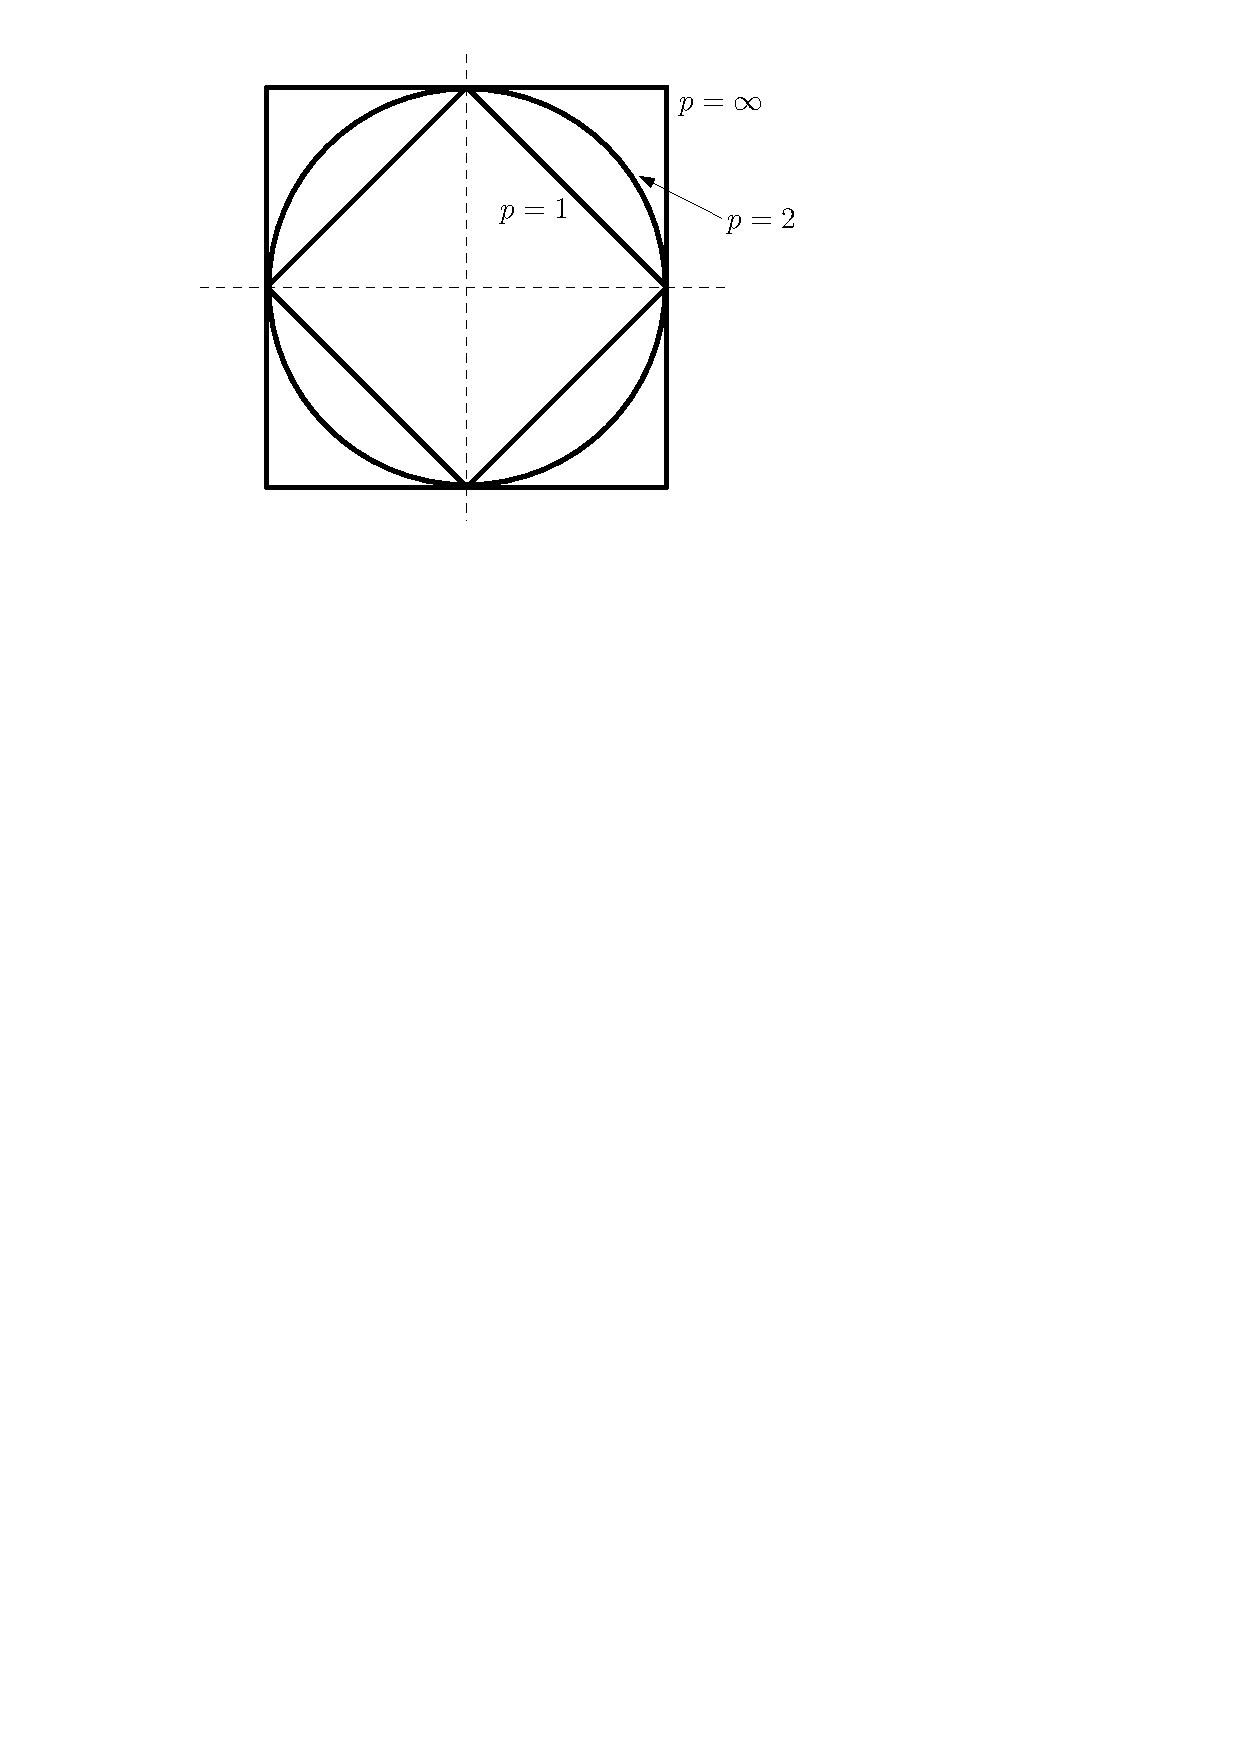
\includegraphics[scale=0.5]{figures/lpnorm1.pdf}
    \caption{Unit balls of $\ell_1$, $\ell_2$ and $\ell_{\infty}$ norms.}
    \label{fig:lpnorm1}
\end{figure}

Notice that all three are indeed closed convex bodies. For $p=2$, we have the ordinary disk. As $p$ decreases to $1$, the unit ball shrinks towards the rhombus. For $p \geq 2$, the unit ball expands towards the square, as $p \rightarrow \infty$. Note that, only the unit balls of $\ell_1$ and $\ell_{\infty}$ have sharp corners -- for any $p>1$ the unit ball is differentiable everywhere.

For $p \in (0,1)$, the mapping \eqref{eq:norm} still defines a metric on $\rd$, which may be useful for some applications, but it no longer defines a norm -- the sub-additive property no longer holds. Consequently, the unit ball is not a convex set, as Figure \ref{fig:lpnorm2} demonstrates.

\begin{figure}[ht]
    \centering
    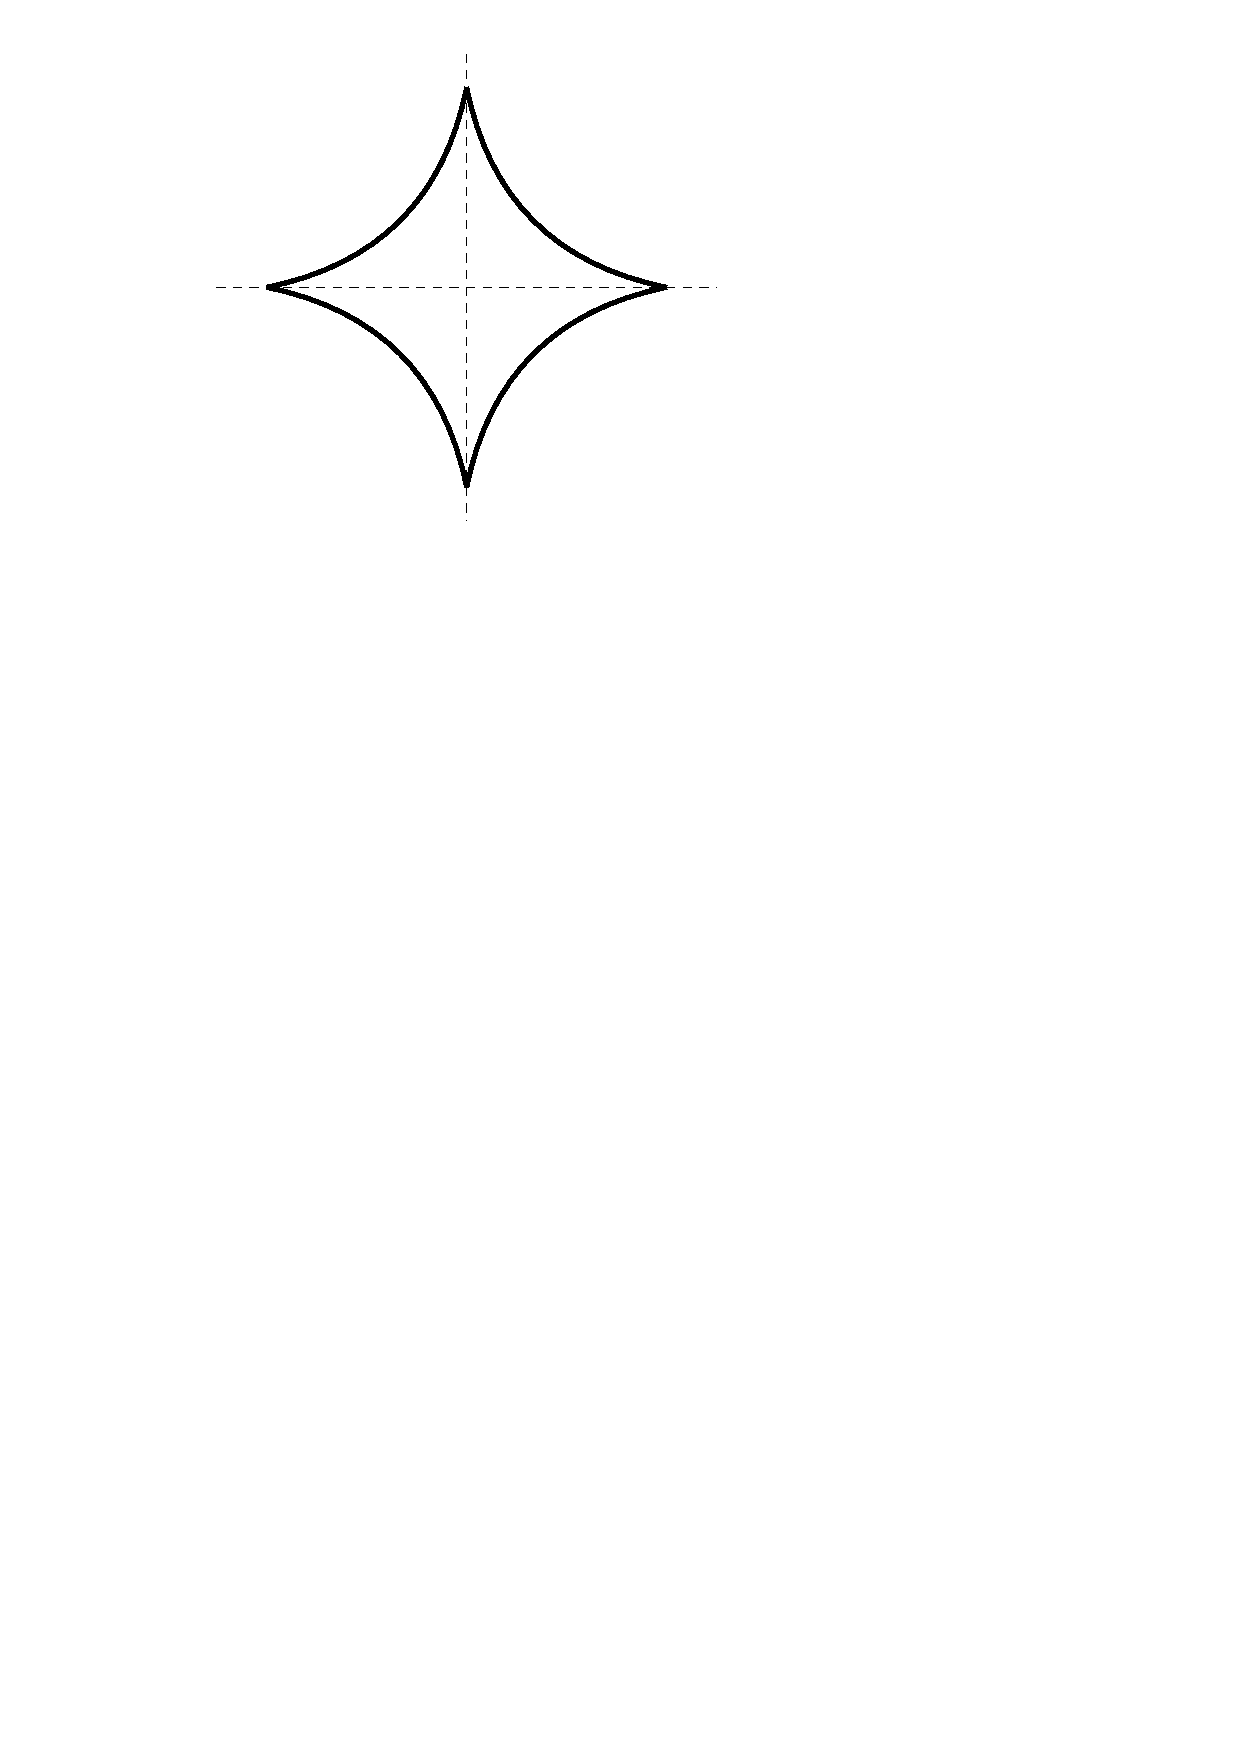
\includegraphics[scale=0.5]{figures/lpnorm2.pdf}
    \caption{The unit ball for $p=2/3$.}
    \label{fig:lpnorm2}
\end{figure}
The next claim provides a connection between $\ell_p$ metrics. 
\begin{claim} \label{ineq:norm}
For any vector $x \in \rd$ and $p>q>0$
\[ \norm{x}_p \leq \norm{x}_q \leq d^{1/q-1/p} \norm{x}_p. \]
\end{claim}
\begin{proof} \renewcommand{\qedsymbol}{}
Appendix \ref{app:holder}.
\end{proof}
%---------------------------------------------------------------------------
\section{Concentration bounds and stable distributions}
%---------------------------------------------------------------------------

Α simple, yet fundamental and tremendously useful inequality in probability theory, is the union bound, also known as Boole's inequality: For any events $A_1. \ldots, A_n$ we have
\[ \prob \left[ \bigcup_{i=1}^n A_i \right] \leq \sum_{i=1}^n \prob[A_i]. \]
The equality holds only if the events are pairwise mutually disjoint.

\subsection*{Concentration inequalities} 
Concentration inequalities provide bounds on how a random variable deviates from some value, typically its expected value. The laws of large numbers of classical probability theory states that sums of independent random variables are, under very mild conditions, close to their expectation with a large probability. Such sums are the most basic examples of random variables concentrated around their mean.

Markov's inequality gives an upper bound for the probability that a non-negative random variable is greater than or equal to some positive constant.  
\begin{theorem}[Markov's inequality]
Let $X$ be a real-valued non-negative random variable. Then for all $\alpha >0$
\begin{equation*}
    \prob[X \geq \alpha] \leq \frac{\EE[X]}{\alpha}.
\end{equation*} 
\end{theorem}
Setting $\alpha = \tilde{\alpha} \EE[X]$, for some $\tilde{\alpha} > 0$, one can rewrite
\[ \prob[X \geq \tilde{\alpha} \EE[X]] \leq \frac{1}{\tilde{\alpha}}. \]

Another popular concentration inequality is the Chernoff bound, which gives exponentially decreasing bounds on tail distributions of sums of independent random variables. Although it is a sharper bound than Markov's inequality, the Chernoff bound requires that the variables be independent – a condition that is not required for Markov's inequality.

The generic Chernoff bound is derived using the \textit{moment generating function}:
\begin{definition}
The moment-generating function of a random variable $X$ is
\[M_X(t) = \EE[\ex^{tX}], \ t \in \mathbb{R}, \]
whenever this expectation exists.
\end{definition}

\begin{theorem} [Generic Chernoff bound]
Let $S$ be the sum of $n$ \textit{independent} random variables, $X_1, \ldots, X_n$ and $\alpha \in \mathbb{R}$. Then, for every $t >0$
\begin{align*}
    \prob[S \geq \alpha] &\leq \ex^{-t\alpha} \cdot \prod_{i=1}^n \EE[\ex^{tX_i}], \\
    \prob[S \leq \alpha] &\leq \ex^{t\alpha} \cdot \prod_{i=1}^n \EE[\ex^{-tX_i}].
\end{align*}
\end{theorem}

\begin{proof}
By Markov's inequality, and since $X_i$'s are independent:
\begin{align*}
    \prob[S \geq \alpha] = \prob[\ex^{tS} \geq \ex^{t\alpha}] \leq \frac{\EE[\ex^{tS}]}{\ex^{t\alpha}} = \ex^{-t\alpha} \cdot \EE \left[ \prod_{i=1}^n \ex^{tX_i} \right] = \ex^{-t\alpha} \cdot \prod_{i=1}^n \EE[\ex^{tX_i}].
\end{align*}
The second inequality is proved similarly.
\end{proof}

Notice that with the Chernoff bound, one can derive a concentration inequality for a sum of independent random variables, by using a bound on the moment generating function.

\subsection*{Stable distributions}
Stable distributions \cite{Zol86} are defined as limits of normalized sums of independent identically distributed variables (an alternate definition follows). The most known example of a stable distribution is Gaussian distribution. However, the class is much wider; for example, it includes heavy-tailed distributions.

\begin{definition}
A distribution $\mathcal{D}$ over $\mathbb{R}$ is called $p$-stable, if there exists $p > 0$ such that for any $d$ real numbers $v_1, \ldots, v_d$ and i.i.d. variables $X_1, \ldots, X_d$ with distribution $\mathcal{D}$, the random variable $\sum_i v_i X_i$ has the same distribution as $X \cdot (\sum_i |v_i|^{p})^{1/p}$, where $X \sim \mathcal{D}$.
\end{definition}
Stable distributions are known to exist for any $p \in (0,2]$. In particular:
\begin{itemize}
    \item The Gaussian distribution ($\mathcal{D}_G$), with density $g(x) = \frac{1}{\sqrt{2 \pi}} \ex^{-x^2/2}$, is $2$-stable.
    \item The Cauchy distribution $(\cauchy)$, with density $c(x) = \frac{1}{\pi} \frac{1}{1 + x^2}$, is $1$-stable.
\end{itemize}

From a practical point of view, despite the lack of closed form density and distribution functions, it is known \cite{CMS76} that one can generate a $p$-stable random variable $X$ by taking
\[ X = \frac{\sin{(p \theta)}}{\cos^{1/p}{\theta}} \left( \frac{\cos{(\theta(1-p))}}{-\ln{r}} \right)^{(1-p)/p},\]
where $\theta$ is uniform on $[-\pi/2, \pi/2]$ and $r$ is uniform on $[0,1]$. Stable distributions have found numerous applications in various fields \cite{Nol18}. In computer science, they are used for sketching and dimension reduction.

The main property of $p$-stable distributions directly translates into a sketching technique. For example, let $0<k<d$ and $f: \rd \rightarrow \rk$, such that for any $v \in \rd$, $f(v)=A \cdot v$, where $A$ is a random $k{\times}d$ matrix, with each entry being an i.i.d.\ variable from a $p$-stable distribution. Let $A_j, j \in [k]$ be the $j$-th row of $A$. Then, $f(v)$ is a tuple of $k$ dot products:
\[ f(v) = (\langle A_1, v \rangle, \ldots, \langle A_k, v \rangle). \]
By the $p$-stability property, $f(v)$ is distributed as
\[ (Y_1 \cdot \norm{v}_p, \ldots, Y_k \cdot \norm{v}_p) =  \norm{v}_p \cdot (Y_1, \ldots, Y_k), \]
where the $Y_j$'s are i.i.d. with $p$-stable distribution. 

Now, one can use $f(v)$, which is termed as the sketch of $v$, to analyze $\norm{v}_p$. In addition, the map $f$ defines a randomized projection of $\rd$ to $\rk$.

%---------------------------------------------------------------------------
\section{Locality-Sensitive Hashing} \label{section:lsh}
%---------------------------------------------------------------------------
The main idea behind LSH, as mentioned in Section \ref{section:prev}, is \textit{random space partitions}, which have the property that a pair of close points (at distance at most $r$) is more likely to belong to the same part than a pair of far points (at distance more than $cr$). Given such a partition, the data structure splits the dataset $P$ accordingly, and, given a query, retrieves all the data points which belong to the same part as the query.

\begin{definition} [Locality-Sensitive Hashing] \label{def:lsh}
Fix a metric space $(X, d_X)$, $r>0$, approximation $c >1$, and a set $U$. Then a distribution $\mathcal{H}$ over maps $h: X \rightarrow U$ is $(r,cr,p_1,p_2)$-sensitive if for any $x,y \in X$
\begin{align*}
    d_X(x,y) \leq r &\implies \prob_{h \sim \mathcal{H}}[h(x) = h(y)] \geq p_1, \\
    d_X(x,y) \geq cr &\implies \prob_{h \sim \mathcal{H}}[h(x) = h(y)] \leq p_2.
\end{align*}
The distribution $\mathcal{H}$ is called LSH family and has quality $\rho = \rho(\mathcal{H}) = \frac{\log{(1/p_1)}}{\log{(1/p_2)}}$.
\end{definition}

An LSH family is meaningful when $p_1 > p_2$, and therefore $\rho < 1$. Notice that LSH mappings are oblivious: they are well-defined over the whole metric space. Hence, data structures based on LSH can naturally work in an online setting with insertions and deletions.

\begin{theorem} [\cite{IM98}]
Let $P \subset (X, d_X)$, $|P|=n$, and let $\mathcal{H}$ be an $(r,cr,p_1,p_2)$-sensitive LSH family for $(X, d_X)$ with quality $\rho$. Then there exists a fully dynamic data structure for $(c,r)$-ANN with space and preprocessing time $O(n^{1+\rho} + dn)$ and query time $O(dn^{\rho})$. The data structure is correct with constant probability.
\end{theorem}

\begin{theorem} [\cite{IM98}]
There exist an $(r,cr,p_1,p_2)$-sensitive LSH family for the Hamming space with quality $\rho = 1/c$.
\end{theorem}
The distribution $\mathcal{H}$ is simply defined as projections on random coordinates: $\mathcal{H} = \{h_i: h_i(x)=x_i, i =1, \ldots,d \}$. This family is $(r,cr,1-r/d,1-cr/d)$-sensitive and therefore, $\rho \leq 1/c$. Note that this LSH family can be extended to the Manhattan ($\ell_1$). 

\begin{theorem} [\cite{AI08}] \label{theorem:lsh2}
There exist an $(r,cr,p_1,p_2)$-sensitive LSH family for the Euclidean metric with quality $\rho = 1/c^2 + o(1)$.
\end{theorem}
This LSH family partitions the space into Euclidean balls. It proceeds in two steps: first it performs a random dimension reduction to dimension $t$, where $t$ is a parameter, and then partitions $\mathbb{R}^t$ into balls.

%---------------------------------------------------------------------------
\section{Doubling sets and covering nets} \label{section:double}
%---------------------------------------------------------------------------
\subsection*{Doubling dimension}
Let's restate the definition in a more rigorous way:
\begin{definition*} 
Let $(X, d_X)$ be a metric space and $B_X(x,r)=\{y \in X: d_X(x,y) \leq r \}$. The {\em doubling constant} of $X$, denoted $\lambda_X$, is the smallest integer $\lambda \geq 1$ such that for any $p \in X$ and $r > 0$, there exist a set $S \subseteq X$ of cardinality at most $\lambda_X$, such that
\[
B_X(p,r) \subseteq \bigcup_{s \in S} B_X(s,r/2).
\]
The \textit{doubling dimension} of $X$ is defined as $\dim(X)=\log{\lambda_X}$.
\end{definition*}

The following properties demonstrate that $\dim(X)$ is a robust and meaningful notion.
\begin{enumerate} \itemsep0em
    \item If $|X|=n$, then $\dim(X) \leq \log n$.
    \item For $X=\rd$ equipped with any norm, $\dim(X) = \Theta(d)$.
    \item If $S \subseteq X$, then $\dim(S) \leq \dim(X)$.
    \item $\dim(X_1 \cup \ldots \cup X_m) \leq \max_i \{ \dim(X_i) \}+ \log m$.
\end{enumerate}

\paragraph{Motivation.} Doubling metrics often occur naturally in practical applications, where the data set $P$ is contained in the union of low-dimensional manifolds lying in some very high-dimensional space $\rd$, and the distance function is some norm of $\rd$. In such cases, algorithms that exploit the doubling dimension of the data set might be superior to algorithms which consider only the structure of the high dimensional host space. 

\subsection*{Exact and approximate \texorpdfstring{$r$}{r}-nets}
Nets play an important role in the study of embeddings, as well as in designing efficient data structures for doubling spaces. The formal definition is followed by an illustration.

\begin{definition} [$r$-net]
Let $(X, d_X)$ be a metric space and $r>0$. A subset $\net \subseteq X$ is called an $r$-net if it satisfies the following properties:
\begin{itemize} \itemsep0em
    \item {\em $r$-Packing}: For every $s, s' \in \net$, $d_X(s,s') > r$.
    \item {\em $r$-Covering}: For every $x \in X$, there exists $s \in \net$ such that $d_X(x,s) \leq r$. 
\end{itemize}
\end{definition}

\begin{figure}[ht]
    \centering
    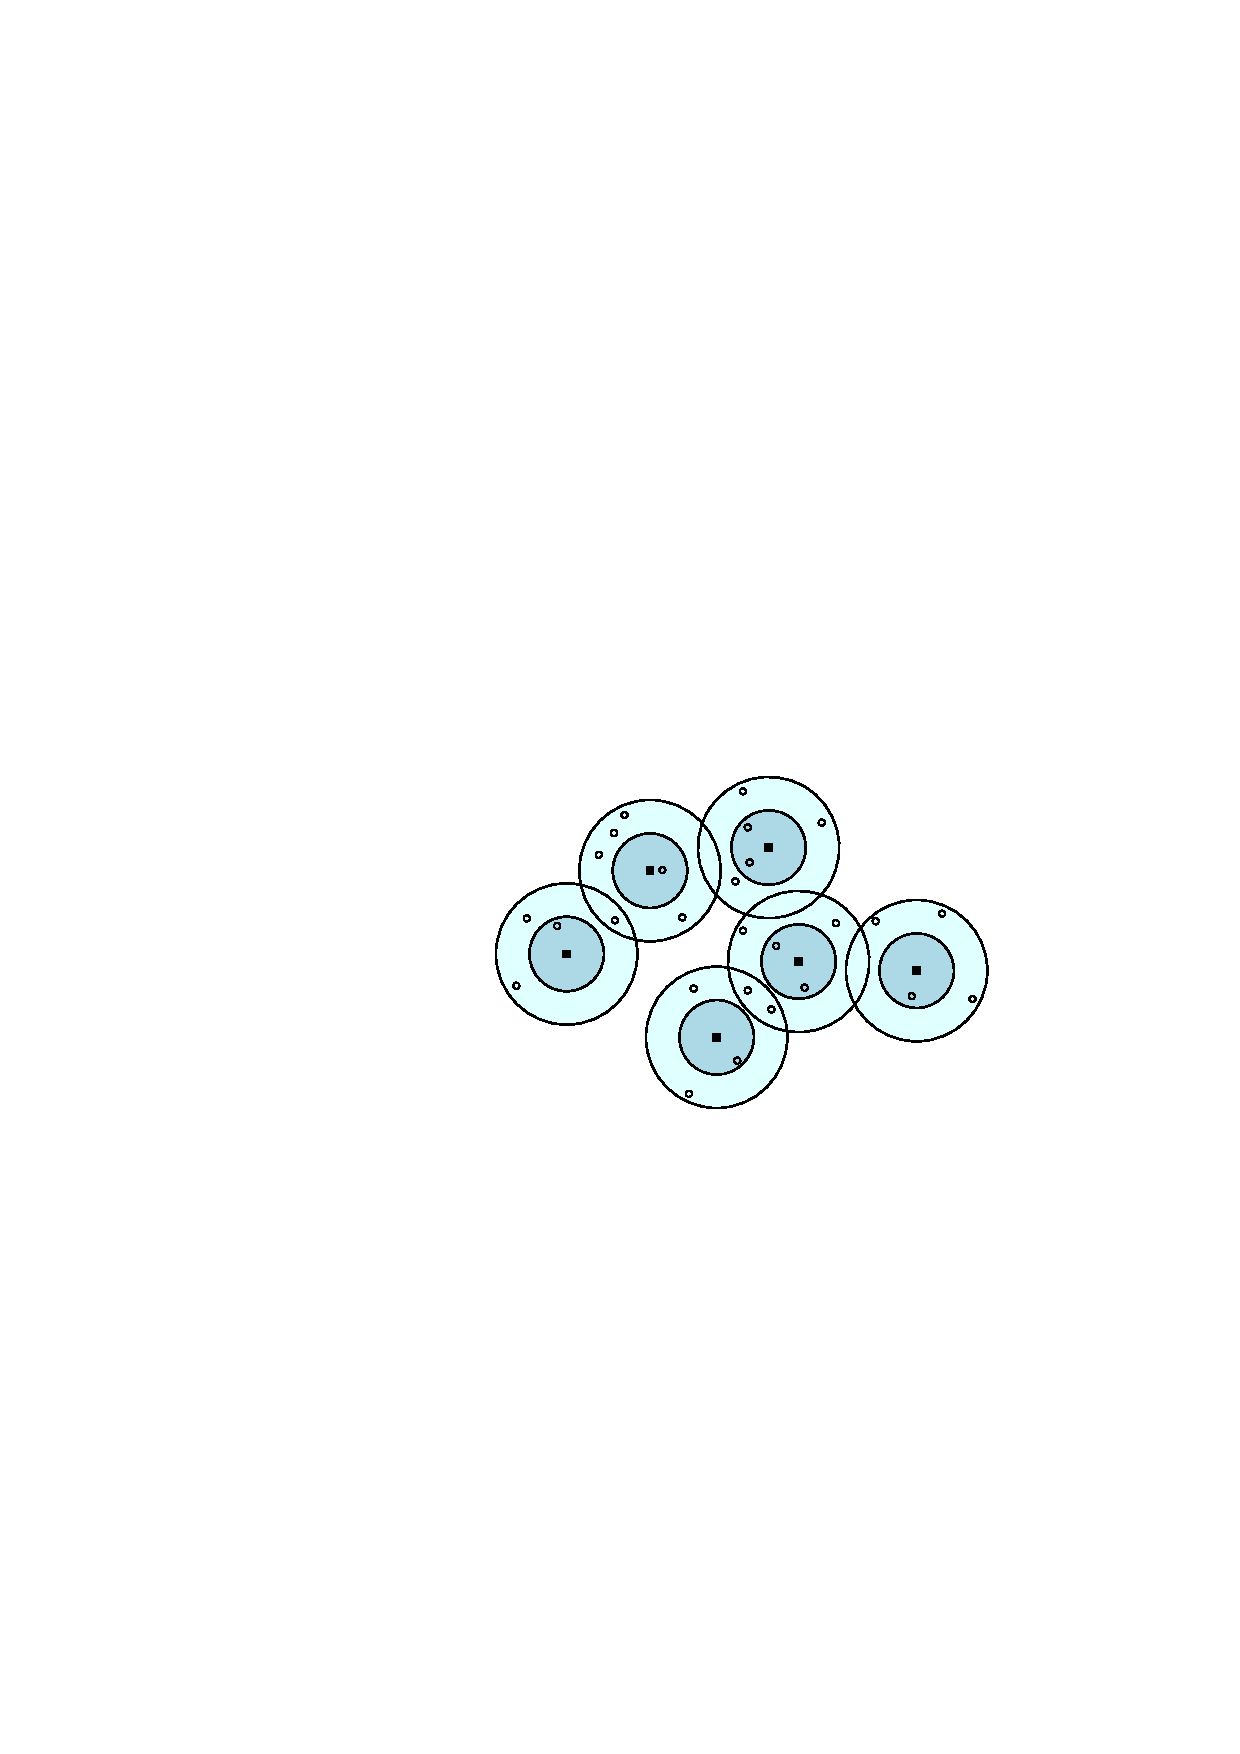
\includegraphics[scale=0.7]{figures/rnet.pdf}
    \caption{An $r$-net of a pointset $P \subset \mathbb{R}^2$. Net points are depicted as squares. The small disks have radius $r/2$ and the large disks have radius $r$. Observe that by the packing property, the small disks are disjoint, and by the covering property, the large disks cover all points of $P$.}
    \label{fig:rnet}
\end{figure}
Nets are ``sparse" representative sets that try to capture the geometry of a metric space. The following lemma demonstrates why doubling spaces and $r$-nets are closely related.
\begin{lemma} \label{lemma:netdouble}
Let $(X, d_X)$ be a metric space of bounded diameter $\Delta$ and doubling constant $\lambda_X$. Let also $\net \subseteq X$ be an $r$-net of $X$. Then
\begin{equation*}
    |\net| \leq \lambda_X^{\lceil \log{(2\Delta/ r)} \rceil}.
\end{equation*}    
\end{lemma}

\begin{proof}
For some $s \in \net$ and $R>0$, let $B_{\net}(s,R) := \{s' \in \net: d_V(s,s') \leq R\}$. Since $\net$ is a subset of $X$, by the definition of $\lambda_X$, there exists a set $S_1 \subseteq \net$ of cardinality at most $\lambda_X$, such that for every $s \in \net$,
\[  \net = B_{\net}(s, \Delta) \subseteq \bigcup_{s' \in S_1} B_{\net}(s', \Delta/2).\]
Applying the definition $k$ times in a recursive fashion, yields a set $S_k \subseteq \net$ of cardinality at most $\lambda_X^k$, such that for every $s \in \net$,
\[  \net \subseteq \bigcup_{s' \in S_k} B_{\net}(s', \Delta/2^k).\]
Therefore,
\[  |\net| \leq \sum_{s' \in S_k} |B_{\net}(s', \Delta/2^k)|.\]
By the packing property of the $r$-net, for every $s \in \net$, $B_{\net}(s,r/2) = \{s\}$.
Hence, for $k = \lceil \log{(2\Delta/ r)} \rceil$,
\[  |\net| \leq \sum_{s' \in S_k} |B_{\net}(s', r/2)| \leq \lambda_X^{\lceil \log{(2\Delta/ r)} \rceil}. \qedhere\]
\end{proof}

For set $P$ of $n$ points in some metric space $(X, d_X)$ and $r>0$, an $r$-net can be computed in $O(n^2)$ time by a greedy algorithm: Pick an arbitrary ordering of the points, $p_1, \ldots, p_n$. Set $\net = \{p_1\}$ and cover all points that are at distance at most $r$ from $p_1$. Continue with $p_2$; if it is covered, proceed to $p_3$, else, add $p_2$ to $\net$ and cover all points within distance $r$ from it. Continue until all points are processed or covered, and return $\net$. 

In \cite{EHS15}, the notion of $r$-nets was extended to $c$-approximate $r$-nets, where the covering property is relaxed. Notice that Lemma \ref{lemma:netdouble} applies to $c$-approximate $r$-nets as well, since only the covering property has changed.
\begin{definition} [$c$-approximate $r$-net]
For $c \geq 1$, $r >0$ and metric space $(X,d_X)$, a $c$-approximate $r$-net of $X$ is a subset $\net \subseteq X$ that satisfies
\begin{itemize} \itemsep0em
    \item {\em $r$-Packing}: For every $s, s' \in \net$, $d_X(s,s') > r$.
    \item {\em $cr$-Covering}: For every $x \in X$, there exists $s \in \net$ such that $d_X(x,s) \leq cr$. 
\end{itemize}
\end{definition}

\begin{theorem} [\cite{EHS15}] \label{theorem:apprnetsl2} 
Let $P\subset \ell_2^d$ such that $|P|=n$. Then, for any $r>0$, $\eps>0$, one can compute a $(1+ \eps)$-approximate $r$-net of $P$ in expected running time $O(\eps^{-2}n^{1+1/(1+\eps)^2+o(1)})$. The result is correct with high probability.
\end{theorem}

The algorithm consists of a Johnson-Lindenstrauss projection as a preprocessing step, and a combination of the greedy algorithm with the LSH family of Theorem \ref{theorem:lsh2}. We use this technique in Section \ref{section:aprnets} to compute approximate nets for the $\ell_1$ norm.

%--------------------------------------------------------
\section{Randomly shifted grids} \label{grids}
%--------------------------------------------------------

Let $w >0$ and $t$ be chosen uniformly at random from the interval $[0,w]$. The function 
\[h_{w, t}(x)=\left\lfloor \frac{x-t}{w} \right\rfloor\]
induces a random partition of the real line into segments of length $w$. Hence, the function 
\[g_{w}(x)=(h_{w,t_1}(x_1),...,h_{w,t_d}(x_d)),\]
for $t_1,\ldots,t_d$ independent uniform random variables in the interval $[0,w)$, 
induces a randomly shifted grid in $\rd$. For a set $X \subseteq \rd$, we denote by $g_{w}(X)$, the image of $X$ on the randomly shifted grid points defined by $g_{w}$. 

\begin{figure}[ht]
    \centering
    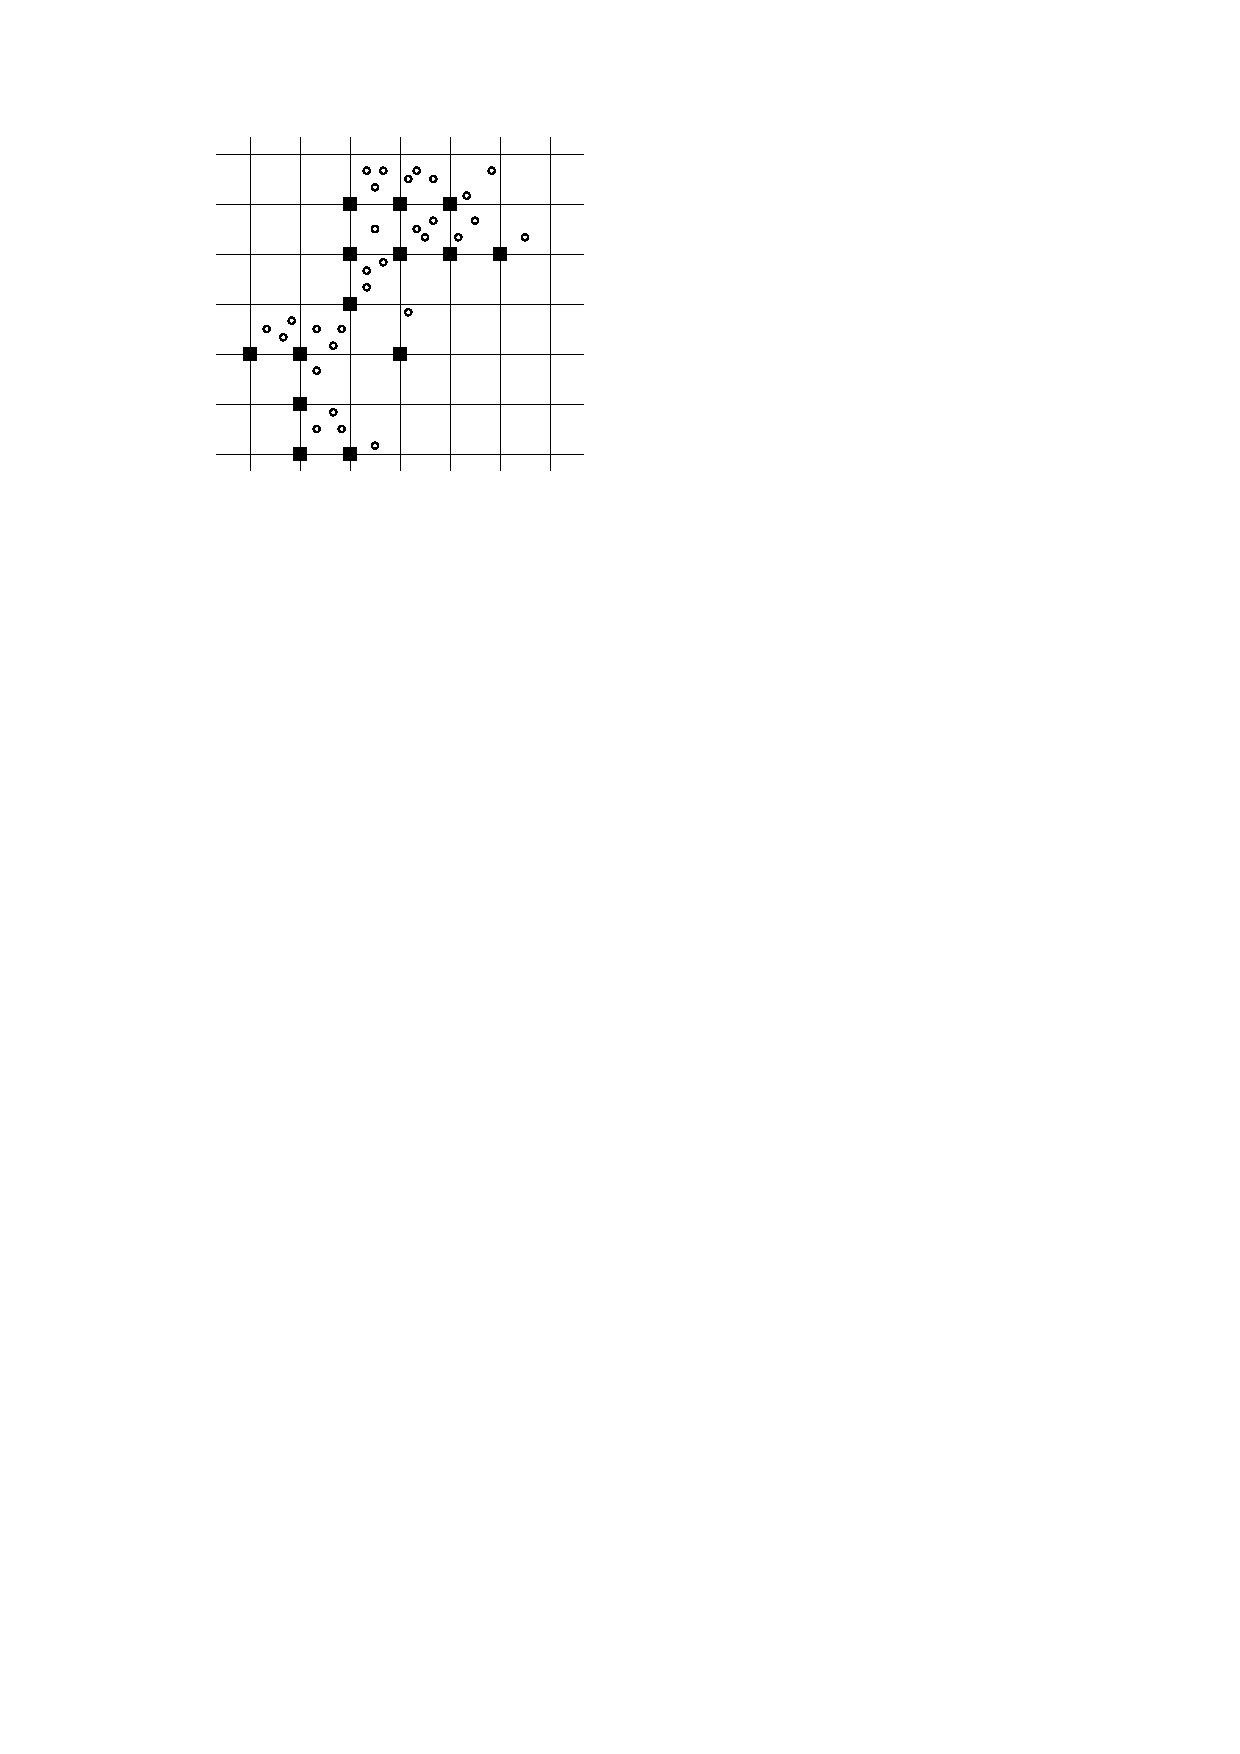
\includegraphics[scale=0.7]{figures/grid2.pdf}
    \caption{A pointset $P$ (circles) and $g_w(P)$ (squares). Each point of $P$ is mapped onto the bottom left point of the cell in which it lies.}
    \label{fig:grid78}
\end{figure}

The next claim concerns the expected number of grid points that are contained in some closed interval.
\begin{claim} \label{claim:1dgrid}
Let $[a,b] \subset \mathbb{R}$ be an interval of length $L>0$ and $w>0$. Then
\[ \EE[|[a,b] \cap h_{w,t}(\mathbb{R})|] = L/w.\]
\end{claim}
\begin{proof}
Let $M = |[a,b] \cap h_{w,t}(\mathbb{R})|$ and assume wlog that $[a,b] = [0,L]$. Think of the case where $t=0$, and then observe how $M$ changes as $t \rightarrow w$. 
\begin{figure}[ht]
    \centering
    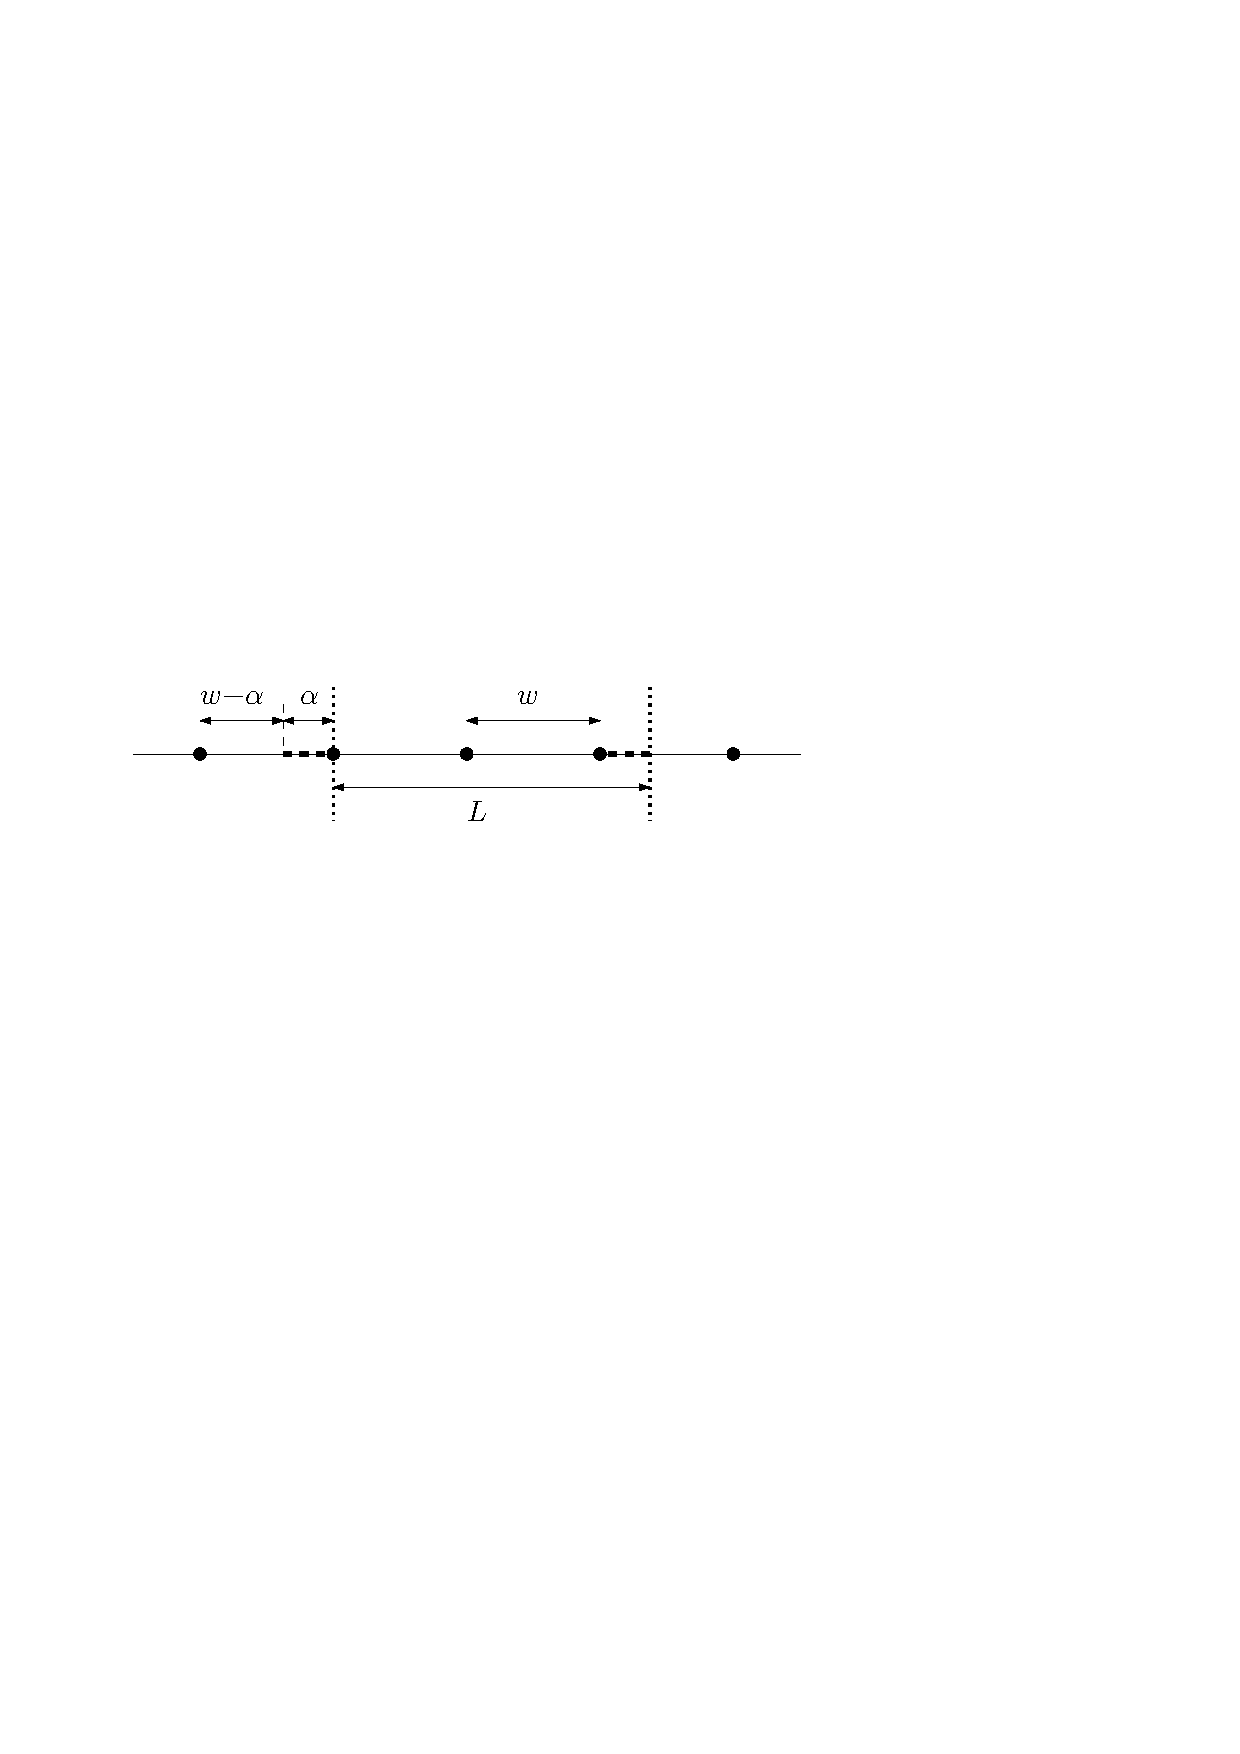
\includegraphics[scale=0.65]{figures/gridline2.pdf}
    \caption{}
    \label{fig:gridline}
\end{figure}

Increasing $t$ corresponds to moving the interval to the left by $t$. Therefore, there exists a threshold $\alpha>0$, such that 
\[
M=
\begin{cases}
\lfloor L/w \rfloor +1, & \text{ if } t \in [0, \alpha]\\
\lfloor L/w \rfloor, & \text{ if } t \in (\alpha, w).
\end{cases}
\]
As we can see in figure \ref{fig:gridline}, $\alpha =L-  \lfloor L/w \rfloor w$. Moreover, since we choose $t$ uniformly in $[0,w)$,
\[
\EE[M] = \frac{\alpha}{w} \left( \left \lfloor \frac{L}{w} \right \rfloor +1 \right) + \frac{(w- \alpha)}{w} \left \lfloor \frac{L}{w} \right \rfloor = \left \lfloor \frac{L}{w} \right \rfloor + \frac{\alpha}{w} = \frac{L}{w}. \qedhere
\]
\end{proof}

Let $B_1(x,r)$ denote the $\ell_1$-ball of radius $r>0$ around a point $x\in \rd$. The next lemma, provides a bound on the expected number of grid points that the ball contains.

\begin{lemma} \label{lemma:dgrid}
For any $x \in \rd$ and $r>0$, we have
\[ \EE[|B_1(x,r) \cap g_w(\rd)|] \leq (1+2r/w)^d.\]
\end{lemma}

\begin{proof}
Let $M := |B_1(x,r) \cap g_w(\rd)|$ and $\cell$ be the total number of grid cells intersecting $B_1(x,r)$. Each grid point corresponds to a grid cell, hence $M$ is bounded by $\cell$. Now, let $\cell_i$ denote the number of grid cells that $B_1(x,r)$ intersects in the axis $i$. Obviously, $\cell \leq \prod_{i \in [d]} \cell_i$ (see Figure \ref{fig:2dgrid}). Therefore,
\[ \EE[M] \leq \EE[\cell] \leq \EE \left[ \prod_{i=1}^d \cell_i \right]. \]

By Claim \ref{claim:1dgrid}, we have that $\EE[\cell_i] = 1+ 2r/w$. Recall that the random shift $t_i$ is independent per axis and so the $\cell_i$'s are also independent. Consequently,

\[ \EE[M] \leq \EE \left[ \prod_{i=1}^d \cell_i \right] = \prod_{i=1}^d \EE[\cell_i] = (1+2r/ w)^d. \qedhere\]
\end{proof}

\begin{figure}[ht]
    \centering
    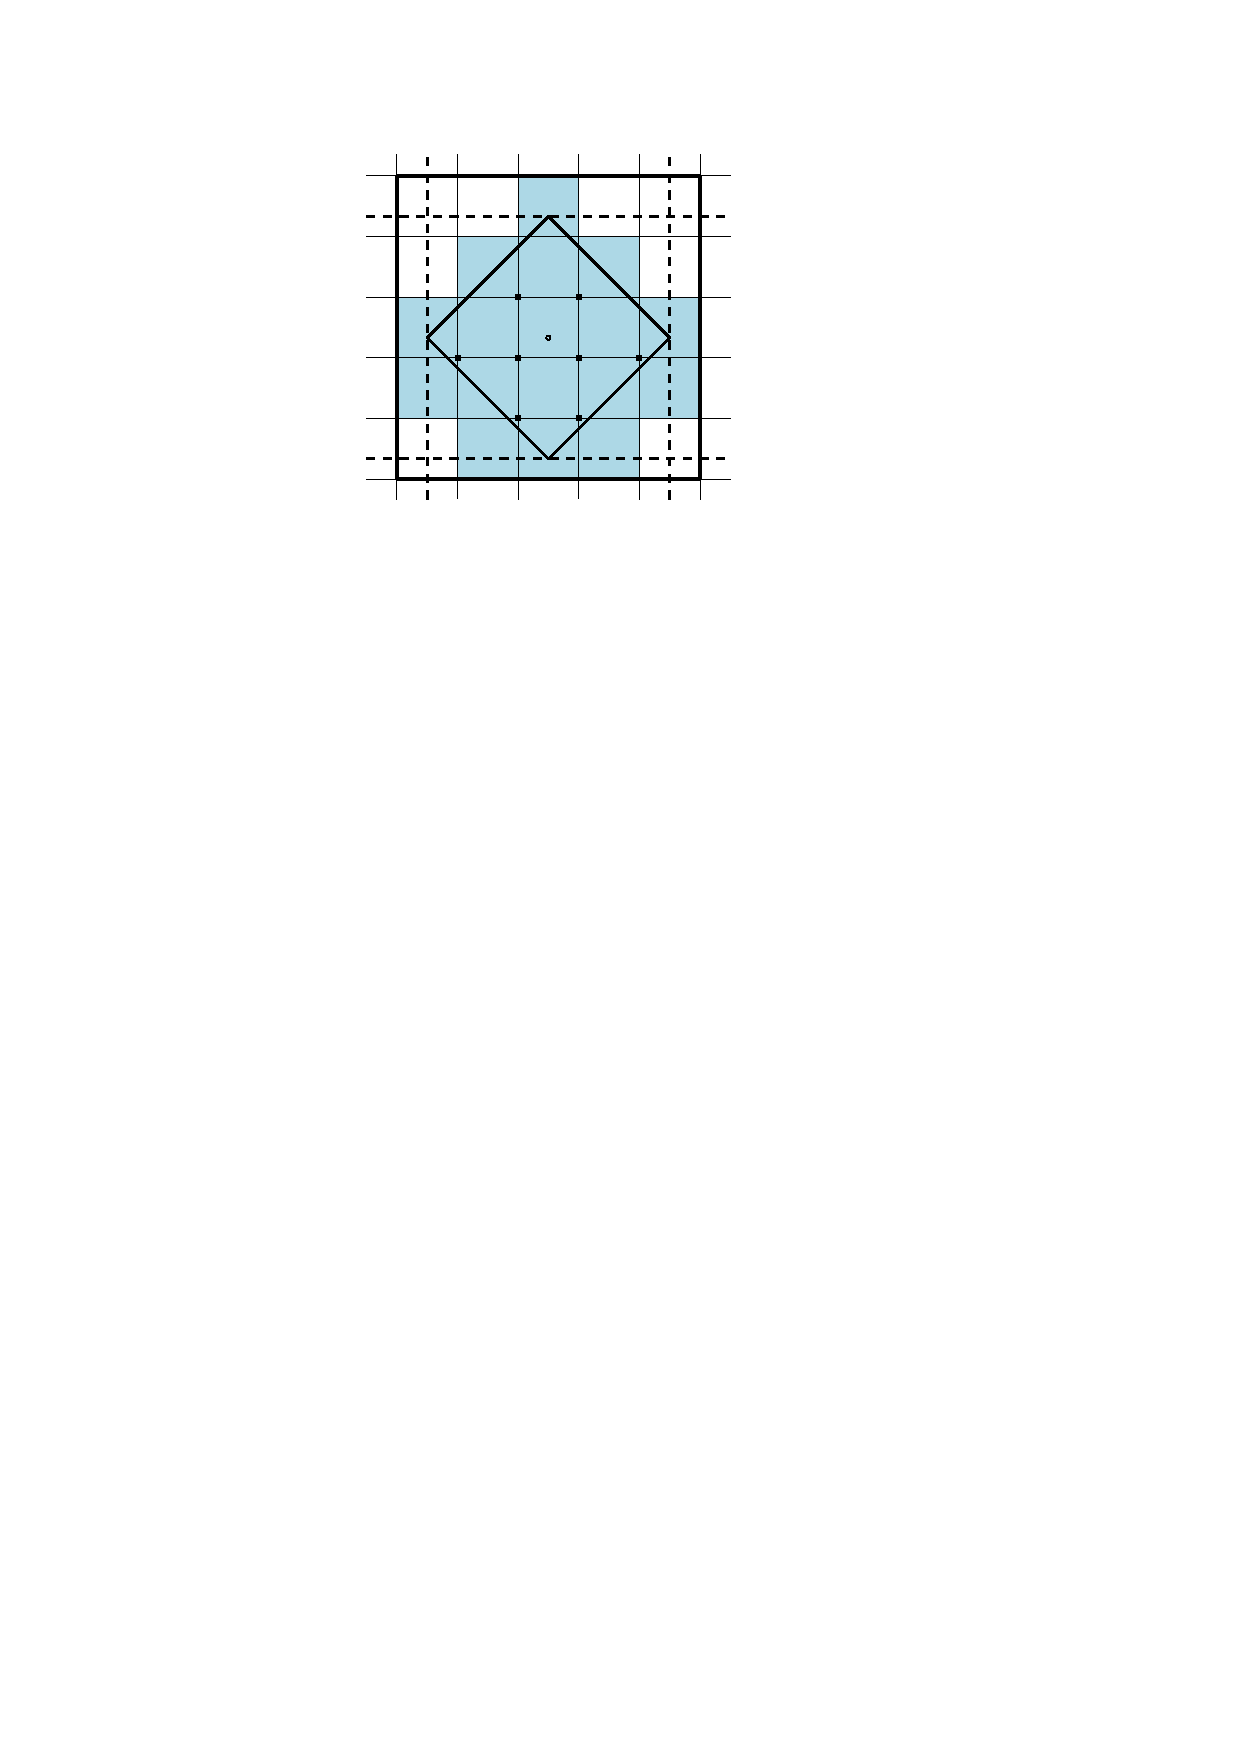
\includegraphics[scale=0.9]{figures/grid2d.pdf}
    \caption{Grid cells intersecting an $\ell_1$ ball.}
    \label{fig:2dgrid}
\end{figure}

Notice that the bound of Lemma \ref{lemma:dgrid} also holds for any $\ell_p$ ball of radius $r$, as the arguments in the proof apply for the $\ell_{\infty}$ ball as well.

%------------------------------------------------------------------------------
\clearpage
\thispagestyle{empty}
\chapter{Randomized embeddings for doubling subsets of \texorpdfstring{$\ell_1$}{L1}}
%---------------------------------------------------------------------------

%---------------------------------------------------------------------------
\section{A concentration bound for sums of Cauchy variables}
%---------------------------------------------------------------------------
In this section, we present a concentration inequality for sums of Cauchy variables, which serves as one of main tools for the analysis.  

Recall the Cauchy distribution, denoted $\cauchy$, with density 
\[ c(x) = \frac{1}{\pi} \frac{1}{1+x^2}. \]
Unlike the Gaussian distribution, the Cauchy distribution has no mean, variance, and moment generating function. However, for $0 < q < 1$, the mean of the $q$th power of the absolute value of a Cauchy random variable can be defined. More specifically, for some $X \sim \cauchy$ we have
\begin{equation*} \label{exphalf}
    \EE \left[ |X|^{1/2} \right] =  \frac{2}{\pi} \int_{0}^{\infty} \frac{\sqrt{x}}{1+x^2} \dx = \frac{2}{\pi} \frac{\pi}{\sqrt{2}} = \sqrt{2}.
\end{equation*}

The following lemma provides a bound for the moment-generating function of $|X|^{1/2}$.
\begin{lemma} \label{lemma:mgf}
Let $X \sim \cauchy$. Then for any $\beta > 1$:
\begin{equation*}
    \EE \left[ \exp{(-\beta |X|^{1/2})} \right] \leq  \frac{2}{\beta}.
\end{equation*}
\end{lemma}

\begin{proof}
For any constant $\beta>0$, we have \footnote{See Appendix \ref{app:integral} for the proof of \eqref{eq:int}.}
\begin{equation} \label{eq:int}
    \int_{0}^{1} \ex^{-\beta x^{1/2}} \dx = \frac{2}{\beta^2}\left(1 - \frac{\beta + 1}{\ex ^{\beta}} \right).
\end{equation}
Moreover,
\begin{align*}
    \ex^{-\beta x^{1/2}} &\leq \ex^{-\beta}, \quad \forall x \geq 1, \beta>0, \\
    \frac{1}{1+x} &\leq 1, \quad \quad \ \forall x \in [0,1].
\end{align*}
Hence, for any $\beta > 1$,
\begin{align*}
    \EE \left[ \exp{(-\beta |X|^{1/2})} \right] &= \int_{-\infty}^{\infty} \ex^{-\beta |x|^{1/2}} \cdot c(x) \dx  \\
    &=  \frac{2}{\pi} \int_{0}^{\infty} \ex^{-\beta x^{1/2}} \cdot \frac{1}{1+x^2} \dx \\
    &=  \frac{2}{\pi} \int_{0}^{1} \ex^{-\beta x^{1/2}} \cdot \frac{1}{1+x^2} \dx + \frac{2}{\pi} \int_{1}^{\infty} \ex^{-\beta x^{1/2}} \cdot \frac{1}{1+x^2} \dx  \\
    &\leq \frac{2}{\pi} \int_{0}^{1} \ex^{-\beta x^{1/2}} \dx + \frac{2}{\pi} \int_{1}^{\infty} \ex^{-\beta} \cdot \frac{1}{1+x^2} \dx \\
    &= \frac{2}{\pi} \cdot \frac{2}{\beta^2}\left(1 - \frac{\beta + 1}{\ex ^{\beta}} \right) +  \frac{1}{2\ex^{\beta}} \\
    &\leq  \frac{4}{\pi \beta^2}+\frac{1}{2\ex^{\beta}} \\
    &\leq  \frac{3}{2 \beta^2}+\frac{1}{2\ex^{\beta}} \\
    &\leq \frac{2}{\beta} . \qedhere
\end{align*}
\end{proof}
Now, consider a collection of $k$ i.i.d.\ Cauchy variables, $X_1,\ldots,X_k$, and let $S := \sum_{j=1}^k |X_j|$. The non-existence of mean and moment generating function of the Cauchy distribution makes it difficult to prove concentration bounds for $S$. Therefore, we study the sum $\tilde{S} := \sum_{j=1}^k |X_j|^{1/2}$ instead:

\begin{lemma} \label{lemma:normineq}
For any $t>0$,
\[ \prob[S \leq t] \leq \prob[\tilde{S} \leq \sqrt{tk}]. \]
\end{lemma}
\begin{proof}
Set $x = (X_1, \ldots, X_k)$ and observe that $S = \norm{x}_1$ and $\tilde{S} = \norm{x}_{1/2}^{1/2}$. Hence, by Claim \ref{ineq:norm} for $p=1$ and $q=1/2$,
\[ S \leq \tilde{S}^2 \leq k \cdot S. \]
Recall that $S$ and $\tilde{S}$ are random variables. Therefore, for any $t>0$, 
\[ ( S \leq t \implies \tilde{S} \leq \sqrt{tk}) \implies \prob[S \leq t] \leq \prob[\tilde{S} \leq \sqrt{tk}]. \qedhere\]
\end{proof}

We use the bound on the moment-generating function, to prove a Chernoff-type concentration bound for $\tilde{S}$, which by Lemma \ref{lemma:normineq} translates directly into a concentration bound for $S$.

\begin{lemma} \label{conc-bound}
For every $D>1$,
\begin{equation*}
    \prob \left [ \tilde{S} \leq \frac{\EE [\tilde{S}]}{D}\right] \leq \left( \frac{10}{D}\right)^k.
\end{equation*}
\end{lemma}
\begin{proof}
Since $X_j$'s are independent, $\EE[\tilde{S}] = \sqrt{2}k$. Then, by Lemma \ref{lemma:mgf} and Markov's inequality, for any $\beta>1$,
\begin{align*}
    \prob \left [ \tilde{S} \leq \frac{\EE [\tilde{S}]}{D}\right] &= \prob \left[  -\beta \tilde{S} \geq  -\beta\cdot  \frac{\EE [\tilde{S}]}{D}\right] \\
    &= \prob \left[  \exp (-\beta \tilde{S}) \geq  \exp \left(-\beta\cdot  \frac{\EE [\tilde{S}]}{D}\right)\right] \\
    &\leq \frac{\EE [\exp (-\beta \tilde{S})]}{\exp (-\beta \EE [\tilde{S}]/D)} \\
    &= \frac{\EE [\exp (-\beta |X_j|^{1/2})]^k}{\exp (-\beta \sqrt{2}k/D)} \\
    &\leq \left(\frac{2}{\beta} \right)^k \cdot \ex^{\sqrt{2} \beta k/D}.
\end{align*}

Setting $\beta=D$ completes the proof. 
\end{proof}

%---------------------------------------------------------------------------
\section{Computing approximate nets in \texorpdfstring{$\ell_1$}{l1}} \label{section:aprnets}
%---------------------------------------------------------------------------
One of our two embeddings requires the computation of an approximate $r$-net. We follow the same idea as in Theorem \ref{theorem:apprnetsl2}, combining the greedy algorithm with an LSH family for the Hamming space.

\begin{theorem} \label{theorem:apprnets} 
Let $P\subset \ell_1^d$ such that $|P|=n$. Then, for any $c>0$, $r>0$, one can compute a $c$-approximate $r$-net of $P$ in time $\tilde{O}(dn^{1+1/c'})$, where $c'=\Omega(c)$. The result is correct with high probability. The algorithm also returns the assignment of each point to one point of the net, which covers it.
\end{theorem}
\begin{proof}
First, we assume $r=1$, since we are able to re-scale the point set. Now, we consider a randomly shifted grid with side-length $2$. 
The probability that two points $p,q\in P$ fall into the same grid cell, is greater than $1-\|p-q\|_1/2$. For each non-empty grid cell we snap points to a grid: each coordinate is rounded to the nearest multiple of $\delta=1/10dc$.
Then, coordinates are multiplied by $1/\delta$ and each point $x=(x_1,\ldots,x_d) \in [2\delta]^d$ is mapped to $\{0,1\}^{2d /\delta}$ by a function $G$ as
\[
G(x)=(g(x_1),\ldots,g(x_d)),
\]
where $g(z)$ is a binary string of $z$ ones followed by $2/\delta -z$ zeros. For any two points $p,q$ in the same grid cell, let $f(p)$,$f(q)$ be the two binary strings which are obtained by the above procedure. Notice that,
\begin{equation*}
\|f(p)-f(q)\|_1\in \left(\frac{2}{\delta}\right) \cdot \|p-q\|_1  \pm 1. 
\end{equation*}
Hence,
\begin{align*}
    \|p-q\|_1 \leq 1 &\implies \|f(p)-f(q)\|_1 \leq \left(\frac{2}{\delta}\right)+1 ,\\[2pt]
    \|p-q\|_1 \geq c &\implies \|f(p)-f(q)\|_1 \geq \left(\frac{2}{\delta}\right)\cdot c-1 .
\end{align*}

Now, we employ the LSH family of \cite{HIM12}, for the Hamming space. After standard concatenation, we can assume that the family is $ (\rho,c'\rho,n^{-1/c'},n^{-1})$-sensitive, where $\rho=\left({2}/{\delta}\right)+1$ and $c'= \Omega(c)$. 

Notice that for the above two-level hashing table we obtain the following guarantees. 
Any two points $p,q\in P$, such that $\|p-q\|_1\leq 1$, fall into the same bucket with probability at least $p_1/2$. Any two points $p,q\in P$, such that $\|p-q\|_1\geq c$, fall into the same bucket with probability at most $p_2$. 

Finally, we independently build $k=\Theta(n^{1/c'} \log n)$ hashtables as above, where the random hash function is defined as a concatenation of the function which maps points to their grid cell id and one LSH function. We pick an arbitrary ordering $p_1,\ldots,p_n$ of the points, and compute the approximate net in a greedy fashion. We start with $p_1$, and we add it to the net. We mark all (unmarked) points which fall at the same bucket with $p_1$, in one of the $k$ hashtables, and are at distance $\leq c r$. Then, we proceed with $p_2$. If $p_2$ is unmarked, then we repeat the above. Otherwise, we proceed with $p_3$. The above iteration stops when all points have been marked. During the procedure, we are able to store one pointer for each point, indicating the center which covered it. 

\textit{Correctness.} The probability that a good pair $p,q$ does not fall into the same bucket for any of the $k$ hashtables is $\leq \left(1-p_1/2\right)^k \leq n^{-10}$. Hence, the packing property holds, and the covering property holds because the above algorithm stops when all points are marked. 

\textit{Running time.} The time to build the $k$ hashtables is $k\cdot n =\tilde{O}(n^{1+1/c'})$. Then, at most $n$ queries are performed: for each query, we investigate $k$ buckets and the expected number of false positives is $\leq k\cdot n^2 \cdot p_2=\tilde{O}(n^{1+1/c'})$. Hence, if we stop after having seen a sufficient amount of false positives, we obtain time complexity $\tilde{O}(n^{1+1/c'})$ and the covering property holds with constant probability. We can repeat the above procedure $O(\log n)$ times to obtain high probability of success. 
\end{proof}

%---------------------------------------------------------------------------
\section{Dimension reduction via approximate nets}
%---------------------------------------------------------------------------
In this section we describe the dimension reduction mapping for the $\ell_1$ norm via $r$-nets. Let $P\subset \ell_1^d$ be a set of $n$ points with doubling constant $\lambda_P$. For some point $x \in \rd$ and $r>0$, we denote with $B_1(x,r)$ the $\ell_1$-ball of radius $r$ around $x$. The embedding is non-linear and is carried out in two steps: Given $P$, $\eps >0$ and $c \geq 1$,

\begin{enumerate} \itemsep0em
    \item we compute a $c$-approximate $(\eps/c)$-net of $P$ with the algorithm of Theorem \ref{theorem:apprnets}. Let $\net$ be the output of the algorithm. In every iteration, a subset $P_s \subseteq P$ is covered by some point $s \in \net$. Let $g: P \rightarrow \net$ be the function that maps every point of $P_s$ to $s$.
    
    \item Then, for every $s \in \mathcal{N}$ and any query point $q \in \ell_1^d$, we apply the linear map of Theorem \ref{theorem:indyk}. That is,  $f(s) = As/T$, where $A$ is a $k{\times}d$ matrix with each element being an i.i.d. Cauchy random variable. Recall that $T$ is a scaling factor such that $T = \Theta(k \log {(k/ \eps)})$.
\end{enumerate}

We define the embedding to be $h = f \circ g$. We apply $h$ for every point in $P$, and only $f$ for any query $q$. It is clear from the properties of the net that $g$ incurs an additive error of $\eps$ on the distances between $q$ and $P$, so it suffices to study the distortion of $f$. By the $1$-stability property of the Cauchy distribution, the $j$-th coordinate of $f(s)$ is distributed as $\norm{s}_1 Y_j$, for some i.i.d.\ $Y_j \sim \cauchy$. Hence, $\norm{f(s)}_1 = \norm{s}_1 \cdot S$ where $S := \sum_{j \in [k]}|Y_j|$.

Our analysis consists of studying separately the following disjoint subsets of $\net$: Points that lie at distance at most $D_0$ from the query and points that lie at distance at least $D_0$, for some $D_0>1$ chosen appropriately. For the former set, we can directly apply Theorem \ref{theorem:indyk}, as it has bounded diameter.

\paragraph{Handling far points.} The next lemma guarantees the low distortion for the points of the latter set, i.e. those that are sufficiently far from the query. We consider the sum of the square roots of each $|Y_j|$, i.e., $\tilde{S} = \sum_j |Y_j|^{1/2}$, in order to utilize the tools of section 3.

\begin{lemma} \label{lemma:farpoints}
Fix a query point $q \in \ell_1^d$. For any $\eps \in (0,1/2)$, $c \geq 1$, $\delta \in (0,1)$, there exists $D_0=O(\log (k/\eps))$ such that  for $k = \Theta \left( \log^{2}{\lambda_P} \cdot \log ( c / \eps) + \log (1/ \delta) \right)$, with probability at least $1 - \delta$,
\begin{equation*}
    \forall s \in \net : \norm{s-q}_1 \geq D_0 \implies \norm{f(s)-f(q)}_1 \geq 4.
    \end{equation*}
\end{lemma}

\begin{proof}
Let $D_0>1$ and assume wlog that the query point lies at the origin ($q = \mbf{0}$). We define the following subsets of $\net$:
\begin{equation*}
    N_i = \{ s \in \mathcal{N} \ | \ D_i \leq \norm{s}_1 < D_{i+1} \}, \ D_i = 2^{2i} D_0, \ i = 0, 1, 2, \ldots
\end{equation*}
Notice that $N_i \subseteq B_1(q, D_{i+1}) \cap \net$. Then, by Lemma \ref{lemma:netdouble} for $r= \eps/c$, $|N_i|$ is at most $\lambda_P^{\lceil \log \left(4cD_{i+1} / \eps \right) \rceil} \leq \lambda_P^{4 \log \left(cD_{i+1} / \eps \right)}$. Therefore, by the union bound, and Lemma \ref{lemma:normineq}
\begin{align*}
    \prob \left[ \exists i \exists s \in N_i : \norm{f(s)}_{1} \leq \frac{4\norm{s}_{1}}{D_i}  \right] &= \prob \left[ \exists i \exists s \in N_i : S \leq \frac{4T}{D_i}  \right]\\
    &\leq \sum_{i=0}^{\infty} |N_i| \prob \left[\tilde{S} \leq \frac{\sqrt{4kT}}{\sqrt{D_i}} \right] \\
    &= \sum_{i=0}^{\infty} |N_i| \prob \left[\tilde{S} \leq \EE[\tilde{S}] \cdot \sqrt{\frac{2T}{k 2^{2i} D_0}} \right]
\end{align*}
For $D_0 =\lceil 800T/k \rceil = \Theta(\log (k/\eps))$ and $k > 4 \cdot \log{\lambda_P} \cdot \log(c D_0/ \eps)+2 \log (2 \lambda_P/\delta) $, by Lemma \ref{conc-bound}:
\begin{align*}
    \sum_{i=0}^{\infty} |N_i| \prob \left[\tilde{S} \leq \frac{\EE[\tilde{S}]}{10 \cdot 2^{i+1}} \right] &\leq \sum_{i=0}^{\infty} \lambda_P^{4 \log{(cD_{i+1}/ \eps)}} \left( \frac{1}{2^{i+1}}\right)^k \\
    &= \sum_{i=0}^{\infty} \frac{ 2^{\log(\lambda_P)({4 \log{(cD_0/ \eps)}+2i+2})}}{ 2^{k(i+1)}} \\
    &\leq \sum_{i=0}^{\infty} \frac{ 2^{\log(\lambda_P) \cdot 4 \log{(cD_0/ \eps)}} \cdot 2^{2\log(\lambda_P) (i+1)}}{ 2^{(4 \cdot \log{\lambda_P} \cdot \log(c D_0/ \eps))(i+1)} \cdot 2^{2 \log (2 \lambda_P/\delta))(i+1)}} \\
    &\leq \sum_{i=0}^{\infty} { 2^{-2 \log (2/\delta))(i+1)} } \\
    &= \sum_{i=0}^{\infty} \left( \frac{\delta^2}{4} \right)^{i} - 1 \\
    &= \frac{\delta^2}{4 - \delta^2} \\
    &\leq \delta.
\end{align*}

Finally, for some large enough constant $C$, we demand
\begin{align*}
    4 \cdot \log{\lambda_P} \cdot \log(c D_0/ \eps)+2 \log (2 \lambda_P/\delta) &< 4( \log{\lambda_P} \cdot \log(c D_0/ \eps)+ \log ( \lambda_P/\delta) ) \\
    &< 8( \log{\lambda_P} \cdot \log(c D_0/ \eps)+ \log ( 1/\delta) ) \\
    &< C( \log{\lambda_P} \cdot \log(c \log k/ \eps)+ \log ( 1/\delta) ) \\
    &< k.
\end{align*}
which is satisfied for $k = \Theta \left( \log^{2}{\lambda_P} \cdot \log ( c / \eps) + \log (1/ \delta) \right)$.
\end{proof}

Now that we handled the (very) far neighbors, we can prove that the mapping satisfies the desirable conditions for a near neighbor-preserving embedding.
\begin{theorem}
\label{theorem:main}
Let $P \subset \ell_1^d$ such that $|P|=n$. For any $\eps < 1/2$ and $c \geq 1$, there is a non-linear randomized embedding $h = f \circ g: \ell_1^d \rightarrow \ell_1^k$ with target dimension $k = \left( \log{\lambda_P} \cdot \log(c / \eps) \right)^{\Theta(1/\eps)} / \zeta(\eps) $, for a function $\zeta(\eps)>0$ depending only on $\eps$, such that for any  $q \in \ell_1^d$ , if there exists $p^{*}\in P$ such that $\|p^{*}-q\|_1 \leq 1$, then with probability $\Omega(\eps)$,
\begin{align*}
    &\norm{h(p^{*}) - f(q)}_1 \leq 1 + 3\eps, \\
    &\forall p\in P: \norm{p-q}_1 > 1+9\eps \implies \norm{h(p) - f(q)}_1 > 1 + 3\eps.
\end{align*}
The set $P$ can be embedded in time $\tilde{O}(d n^{1+1/ \Omega(c)})$, and any query $q\in \ell_1^d$ can be embedded in time $O(dk)$.
\end{theorem}
\begin{proof}
Let $D_0 = \Theta(\log (k/\eps))$ and assume for simplicity (wlog) that $q=\mbf{0}$. Then, by Lemma \ref{lemma:farpoints} for $k = \Theta \left( \log^{2}{\lambda_P} \cdot \log ( c / \eps)  \right)$, with probability at least $1- \eps/5$
\begin{equation*}
    \forall p \in P : \norm{p-q}_1 \geq D_0 + \eps \implies \norm{h(p) - f(q)}_1 \geq 4.
\end{equation*}

By Theorem \ref{theorem:indyk} for $\gamma = \eps/10$ and $\delta = \eps/ (5\lambda_P^{8\log{(c D_0 / \eps)}})$, with probability at least $1-\eps/5$
\begin{align*}
\forall p\in P: \norm{p-q}_1 \in (1+9\eps, D_0+ \eps)  \implies \norm{h(p) - f(q)}_1 &\geq (1 + 8\eps)(1 - \eps) \\
&> 1 + 3\eps.
\end{align*}
Moreover,
\[
\prob \big[\norm{h(p^*) - f(q)}_1 \leq 1 + 3\eps  \big] \geq 1 -\frac{1+ \eps/10}{1+ \varepsilon} \geq 1 - (1 - \eps/2).
\]
The target dimension then, needs to satisfy
\begin{align*}
    k \geq \frac{\big( \ln{ ( 5\lambda_P^{8\log{(c D_0 / \eps)}} / \eps ) } \big) ^{2/\eps}}{ \zeta(\eps)} = \frac{\big( \Theta ( \log \log k  \cdot \log{\lambda_P} + \log{\lambda_P} \cdot \ln(c / \eps) ) \big) ^{2/\eps}}{ \zeta(\eps)}
\end{align*}
Hence, for $k = \left( \log{\lambda_P} \cdot \log(c / \eps) \right)^{\Theta(1/\eps)} / \zeta(\eps) $ we achieve total probability of success $\Omega(\eps)$, which completes the proof.
\end{proof}

%---------------------------------------------------------------------------
\section{Dimension reduction via randomly shifted grids}
%---------------------------------------------------------------------------
In this section, we present a simplified embedding which grids instead of nets. 
Recall the randomly shifted grid function
\[g_{w}(x)=\left(\left\lfloor \frac{x_1-t_1}{w} \right\rfloor,...,\left\lfloor \frac{x_d-t_d}{w} \right\rfloor \right),\]
where $t_1,\ldots,t_d$ independent uniform random variables in the interval $[0,w]$. 
induces a randomly shifted grid in $\rd$.

Now, let $P \subset \ell_1^d$ be a set of $n$ points with doubling constant $\lambda_P$, $q \in \ell_1^d$ a query point, and $\eps>0$. The embedding is similar as before: First, we compute $\mathcal{G} := g_{\eps /d}(P)$, and then we randomly project $\grid$ and $q$ with $f$, as in Theorem \ref{theorem:indyk}.

By choosing side length $w= \eps /d$, we have that the $\ell_1$-diameter of each cell is $\eps$, and therefore $\grid$ is an $\eps$-covering set of $P$. That is, every point $p \in P$ lies within distance $\eps$ from some point in $\grid$. 

\section*{Properties of $\grid$.} 
We can bound the number of points of $\grid$ that lie inside a bounded ball around the query, using the doubling constant:
\begin{lemma} \label{lemma:grid1}
Let $R>1$ and $P' := B_1(q,R) \cap P$. Then, for $w=\eps/d$
\[ \EE \left[|g_{w}(P')|\right] \leq 8 \lambda_P^{2\log (dR/\eps)}. \] 
\end{lemma}
\begin{proof}
By the doubling constant, there exists a set of balls of radius $\eps/d^2$ centered at points in $P'$, of cardinality at most $\lambda_P^{2\log (d R/\eps)}$ which covers $P'$. By Lemma \ref{lemma:dgrid}, the expected number of grid points contained in each ball is at most
\[\big(1+2(\eps/ d^2)/ (\eps /d) \big)^d = (1+2/d)^d \leq \ex^2.\] 
Hence, the proof follows by linearity of expectation.
\end{proof}

The next lemma shows that with constant probability, the growth on the number of representatives, as we move away from $q$, is bounded. 

\begin{lemma} \label{lemma:grid2}
Let $\{D_i\}_{i \in \mathbb{N}}$ be a sequence of radii such that for any $i$: $D_{i+1}=4 \cdot D_i$, and let $A_i$ be the points of $g_w(P)$ within distance $D_{i+1} = 2^{2(i+1)} D_0$ from $q$. Then, with probability at least $1/3$,
\[
\forall i\in \{-1,0,\ldots\}: |A_i| \leq 4^{i+3} \lambda_P^{2\log (2d D_{i+1}/\eps)}.
\]
\end{lemma}

\begin{proof}
By Lemma \ref{lemma:grid1}, $\EE[ |A_i|] \leq 8 \lambda_P^{2\log (2d D_{i+1}/\eps)}$ for every $i\in \{-1,0,\ldots\}$. Then, a union bound followed by Markov's inequality yields
\begin{equation*}
    \prob \left[ \exists i \in \{0,1,\ldots\} : |A_i| \geq {4^{i+1}} \EE[ |A_i|] \right] \leq  1/3.
\end{equation*}
In addition,
\begin{equation*}
    \prob \left[  |A_{-1}| \geq 4 \EE[ |A_i|] \right] \leq  1/4. \qedhere
\end{equation*}
\end{proof}

\section*{Embedding analysis}
The analysis is the same as with approximate nets; first we handle the representatives the lie sufficiently far from the query, and we invoke Theorem \ref{theorem:indyk} for the rest.

The next lemma is analogous to Lemma \ref{lemma:farpoints}.
\begin{lemma} \label{lemma:farpointsgrid}
Fix a query point $q \in \ell_1^d$. For any $\eps < 1/2$, $\delta \in (0,1)$, there exists $D_0=O(\log (k/\eps))$ such that  for $k = \Theta \left( \log^{2}{\lambda_P} \cdot \log ( d / \eps) + \log (1/ \delta) \right)$, with probability at least $1 - \delta$,
\begin{equation*}
    \forall s \in \grid : \norm{s-q}_1 \geq D_0 \implies \norm{f(s)-f(q))}_1 \geq 4.
\end{equation*}
\end{lemma}

\begin{proof}
Let $D_0>1$ and assume wlog that the query point lies at the origin ($q = \mbf{0}$). We define the following subsets of $\net$:
\begin{equation*}
    G_i = \{ s \in \grid \ | \ D_i \leq \norm{s}_1 < D_{i+1} \}, \ D_i = 2^{2i} D_0, \ i = 0, 1, 2, \ldots
\end{equation*}
Notice that $G_i \subseteq B_1(q, D_{i+1}) \cap \grid$. Then, by Lemma \ref{lemma:grid2}, with constant probability,
\[\forall i: |G_i| \leq 4^{i+3} \lambda_P^{2\log (2d D_{i+1}/\eps)}. \]
Therefore, by the union bound, and Lemma \ref{lemma:normineq}
\begin{align*}
    \prob \left[ \exists i \exists s \in G_i : \norm{f(s)}_{1} \leq \frac{4\norm{s}_{1}}{D_i}  \right] &= \prob \left[ \exists i \exists s \in G_i : S \leq \frac{4T}{D_i}  \right]\\
    &\leq \sum_{i=0}^{\infty} |G_i| \prob \left[\tilde{S} \leq \frac{\sqrt{4kT}}{\sqrt{D_i}} \right] \\
    &= \sum_{i=0}^{\infty} |G_i| \prob \left[\tilde{S} \leq \EE[\tilde{S}] \cdot \sqrt{\frac{2T}{k 2^{2i} D_0}} \right]
\end{align*}
For $k > 2\log{\lambda_P} \cdot \log(2d D_0/ \eps)+4 \log (2 \lambda_P/\delta) +6$ and $D_0 =\lceil 800T/k \rceil = \Theta(\log (k/\eps))$, by Lemma \ref{conc-bound}:
\begin{align*}
    \sum_{i=0}^{\infty} |G_i| \prob \left[\tilde{S} \leq \frac{\EE[\tilde{S}]}{10 \cdot 2^{i+1}} \right] &\leq \sum_{i=0}^{\infty} 4^{i+3} \lambda_P ^ {2\log (2d D_{i+1}/\eps )} \left( \frac{1}{2^{i+1}} \right)^k. \\
    &= \sum_{i=0}^{\infty} \frac{ 2^{2\log(\lambda_P)({\log{(2d D_0/ \eps)}+2i+2}) + 2i + 6}}{ 2^{k(i+1)}} \\
    &\leq \sum_{i=0}^{\infty} \frac{ 2^{2\log(\lambda_P) \cdot \log{(2d D_0/ \eps)}} \cdot 2^{4\log(\lambda_P) (i+1)} \cdot 2^{2i+6}}{ 2^{[\log(\lambda_P) \cdot \log{(2d D_0/ \eps)} + 4 \log (2 \lambda_P/\delta) + 6](i+1)}} \\
    &\leq \sum_{i=0}^{\infty} { 2^{-2 \log (4/\delta)(i+1)} } \\
    &= \sum_{i=0}^{\infty} \left( \frac{\delta^4}{16} \right)^{i} - 1 \\
    &= \frac{\delta^4}{16 - \delta^4} \\
    &\leq \delta.
\end{align*}

For some large enough constant $C$, we demand
\begin{align*}
    2\log{\lambda_P} \cdot \log(2d D_0/ \eps)+4 \log (2 \lambda_P/\delta) + 6 
    &< 8[ \log{\lambda_P} \cdot \log(d D_0/ \eps)+ \log ( \lambda_P/\delta) ] \\
    &< 16[ \log{\lambda_P} \cdot \log(d D_0/ \eps)+ \log ( 1/\delta) ] \\
    &< C[ \log{\lambda_P} \cdot \log(d \log k/ \eps)+ \log ( 1/\delta) ] \\
    &< k.
\end{align*}
which is satisfied for $k = \Theta \left( \log^{2}{\lambda_P} \cdot \log ( d/ \eps) + \log (1/ \delta) \right)$.
\end{proof}

Finally, we prove that the embedding is $(1{+}6\eps)$-Near neighbor-preserving, with probability of correctness $\Omega(\eps)$. We follow the same reasoning as in the proof of Theorem \ref{theorem:main}.
\begin{theorem}
\label{theorem:second}
Let $P\subset \ell_1^d$ such that $|P|=n$. 
For any $\eps < 1/2$, there is a non-linear randomized embedding $h': \ell_1^d \rightarrow \ell_1^k$, where $k = \left( \log{\lambda_P} \cdot \log(d / \eps) \right)^{\Theta(1/\eps)} / \zeta(\eps)$, for a function $\zeta(\eps)>0$ depending only on $\eps$, such that for any  $q \in \ell_1^d$ , if there exists $p^{*}\in P$ such that $\|p^{*}-q\|_1 \leq 1$, then with probability $\Omega(\eps)$,
\begin{align*}
    &\norm{h'(p^{*}) - f(q)}_1 \leq 1 + 3\eps, \\
    &\forall p\in P: \norm{p-q}_1 > 1+9\eps \implies \norm{h'(p) - f(q)}_1 > 1 + 3\eps.
\end{align*}
Any point can be embedded in time $O(dk)$.
\end{theorem}

\begin{proof}
Let $h' = f \circ g_{\eps/d}$, where $f$ is the randomized linear map defined in section 4. As before, we apply $h'$ for every point in $P$, and only $f$ for queries. Note that the randomly shifted grid incurs an additive error of $\eps$ in the distances between $q$ and $P$.

Let $D_0 = \Theta(\log (k/\eps))$ and assume for simplicity (wlog) that $q=\mbf{0}$. Then, by Lemma \ref{lemma:farpointsgrid}, for $k = \Theta \left( \log^{2}{\lambda_P} \cdot \log (d / \eps)  \right)$, with probability at least $1- \eps/5$
\begin{equation*}
    \forall p \in P : \norm{p-q}_1 \geq D_0 + \eps \implies \norm{h(p) - f(q)}_1 \geq 4.
\end{equation*}

Now, we are able to use Theorem \ref{theorem:indyk} for points which are at distance at most $D_0 + \eps$ from $q$, and the near neighbor. By Lemma \ref{lemma:grid2}, with constant probability, the number of grid points at distance $\leq D_0 + \eps$, is at most $32\cdot \lambda_P^{4 \log (dD_0/\eps)}$. Hence, by Theorem \ref{theorem:indyk} for $\gamma = \eps/10$ and $\delta = \eps/ (160\lambda_P^{4\log{(d D_0 / \eps)}})$, with probability at least $1-\eps/5$
\[ \forall p\in P: \norm{p-q}_1 \in (1+9\eps, D_0+ \eps)  \implies \norm{h(p) - f(q)}_1 > 1 + 3\eps. \]
Moreover, with probability at least $\eps/2$
\[
\norm{h'(p^*) - f(q)}_1 \leq 1 + 3\eps.
\]
As in Theorem \ref{theorem:main}, the target dimension needs to satisfy
\begin{align*}
    k \geq \frac{\big( \ln{ ( 160\lambda_P^{4\log{(d D_0 / \eps)}} / \eps ) } \big) ^{2/\eps}}{ \zeta(\eps)} = \frac{\big( \Theta ( \log \log k  \cdot \log{\lambda_P} + \log{\lambda_P} \cdot \ln(d / \eps) ) \big) ^{2/\eps}}{ \zeta(\eps)}
\end{align*}
Hence, for $k = \left( \log{\lambda_P} \cdot \log(d / \eps) \right)^{\Theta(1/\eps)} / \zeta(\eps) $ we achieve total probability of success $\Omega(\eps)$.
\end{proof}


%------------------------------------------------------------------------------
\clearpage
\thispagestyle{empty}
\chapter{Conclusion}
%-----------------------------------------------------------------------------
\section*{Discussion on results}
The results in this thesis show that efficient dimensionality reduction for doubling subsets of $\ell_1$ is possible, in the context of ANN searching. We presented two versions of a non-linear, randomized embedding. In each version, we represent the pointset with a covering set, and then randomly project this set and any query. The embedding is $(1{+}6\eps)$-near neighbor-preserving, with probability of correctness $\Omega(\eps)$. In the first version--Theorem \ref{theorem:main}--we used approximate nets as the representative set, while the second version--Theorem \ref{theorem:second}--considers randomly shifted grids instead. The following table compares target dimension and computation time.
{ \renewcommand{\arraystretch}{1.4}
\begin{center}
\begin{tabular}{|c|c|c|}
\hline
Embedding & Target dimension &  Computation time  \\
\hline 
Theorem \ref{theorem:main}  & $k = \left( \log{\lambda_P} \cdot \log(\mbf{c} / \eps) \right)^{\Theta(1/\eps)} / \zeta(\eps) $ &  $\tilde{O}(dn^{1+1/ \Omega(c)})$ \\
\hline
Theorem \ref{theorem:second} & $k = \left( \log{\lambda_P} \cdot \log(\mbf{d} / \eps) \right)^{\Theta(1/\eps)} / \zeta(\eps) $  &  $O(dkn)$  \\
\hline 
\end{tabular}
\end{center}
}
Theorem \ref{theorem:main} provides with a trade-off between the preprocessing time required and the target dimension, via the parameter $c >1$. For example, for $c=O(1)$, target dimension depends only on $\log{\lambda_P}$ and $\eps$, and preprocessing time is $\tilde{O}(dn^{1+\rho})$, for $\rho <1$. Setting, $c = \log n$, reduces the preprocess to near linear, $\tilde{O}(dn^{1+o(1)})$, but $k$ becomes polynomial in $\log \log n$.

On the other hand, Theorem \ref{theorem:second} has the advantage of fast preprocessing; any point can be embedded in $O(dk)$ time. In addition, the embedding is oblivious to the pointset, as it is well defined on the grid, and may also be of practical interest since it is very easy to implement. However, the target dimension now depends on $\log d$ instead of $\log c$. For near-linear preprocessing, Theorem \ref{theorem:second} is obviously stronger than Theorem \ref{theorem:main} when $d = \mathrm{polylog}(n)$, as we can achieve the same target dimension with exact linear preprocessing time.

Notice that any potential improvements to Theorem \ref{theorem:indyk} could lead to improvements of Theorems \ref{theorem:main} and \ref{theorem:second}. The target dimension in both theorems derives from a direct application of Theorem \ref{theorem:indyk} to the representative points which lie inside a bounding ball centered at the query.

\section*{Algorithmic implications}
Our embedding can be combined with the bucketing method of \cite{HIM12} for the $(1{+} \eps)$-ANN problem in $\ell_1^d$, admitting better space bounds, while preserving the support of fast queries. This data structure requires preprocessing time and space $O(n){\times}O(1/ \eps)^d$ and has query time $O(d)$. Space and preprocessing bounds can be improved to $n^{O{(\log (1/ \eps)/ \eps^2)}}$, with slightly slower $O(d \cdot \log n / \eps^2)$ query time, for general subsets of $\ell_1$. This is done via a JL-like dimension reduction, where the points are first mapped to the Hamming space, which is isometric to $\ell_2$. 

However, for subsets of $\ell_1$ of fixed doubling dimension, one can combine the general bucketing data structure with the embedding of Theorem \ref{theorem:main}, improving upon the bounds obtained by the JL-like embedding, both in space and query time. The following table sums up the comparison.
{ \renewcommand{\arraystretch}{1.4}
\begin{center}
\begin{tabular}{|c|c|c|c|}
\hline
 & JL & Thm \ref{theorem:main} ($c{=}\log n $) & Thm \ref{theorem:main} ($c{=} O(1)$) \\
\hline 
Preprocess  & $n^{O{(\log (\frac{1}{\eps})/ \eps^2)}}$ &  $ \tilde{O}(dn^{1+ o(1)})$ & $ \tilde{O}(dn^{1+ 1/c})$\\
\hline
Space & $n^{O{(\log (\frac{1}{\eps})/ \eps^2)}}$ & $n^{1+ o(1)}$ & $n^{1+ o(1)}$\\
\hline 
Query & $O(d \cdot \log{n} / \eps^2)$  &  $O(d){\times}(\log \log{n})^{O(1/ \eps)}$ & $O(d){\times}(\log (\frac{1}{\eps}))^{O(1/ \eps)}$\\
\hline
\end{tabular}
\end{center}
}

\section*{Open Questions}
An immediate open question is whether better bounds on the target dimension can be proved for the embedding of Theorem \ref{theorem:indyk}. As already mentioned, a positive answer would imply better bounds for Theorems \ref{theorem:main} and \ref{theorem:second} as well. Moreover, an analysis of our embedding which does not rely on the employment of Theorem \ref{theorem:indyk}, might also be of interest.

Stable distributions have been used in designing LSH families and non-linear range embeddings for $\ell_p$ norms, with provable guarantees. An interesting open problem then is whether the linear mapping \`{a} la Johnson-Lindenstrauss can be proven to be NN-preserving for general (or even doubling) subsets of $\ell_p$, $p \in (0,2]$, by substituting the Gaussian matrix with a matrix whose elements are i.i.d.\ $p$-stable variables.

%Another long-standing open problem is to overcome the lower bounds of linear embeddings in $\ell_1$, with randomized \textit{non-linear} bi-Lipschitz embeddings of bounded distortion.

%---------------------
% APPENDICES
%--------------------
\clearpage
\thispagestyle{empty}
%\addappheadtotoc
\appendix
\phantomsection
\chapter*{Appendices}
\noappendicestocpagenum
\addcontentsline{toc}{chapter}{Appendices}
\renewcommand{\thesection}{\Alph{section}}

\section{Proof of Claim 2.2} \label{app:holder}
\begin{claim*}
For any vector $x \in \rd$ and $p>q>0$
\[ \norm{x}_p \leq \norm{x}_q \leq d^{1/q-1/p} \norm{x}_p. \]
\end{claim*}
\begin{proof}
We start with the left part of the inequality by showing that $\norm{x}_p \leq \norm{x}_q$.
If $x = \mbf{0}$, its obviously true. Otherwise, let $y_i = |x_i| / \norm{x}_p \leq 1$, for every $i \in [d]$. Therefore,
\[ \forall i \in [d]: y_i^p \leq y_i^q \implies 1 \leq \norm{y}_q \implies \norm{x}_p \leq \norm{x}_q.\]

For the right part of the inequality, we invoke H\"{o}lder's Inequality: Let $r \in [1, \infty)$. Then for any $a,b \in \rd$
\[ \sum_{i=1}^d |a_i b_i| \leq \left( \sum_{i=1}^d |a_i|^r \right)^{1/r} \left( \sum_{i=1}^d |b_i|^{\frac{r}{r-1}} \right)^{1-1/r}. \] 
Now, set $r=p/q>1$, $a = (|x_1|^q, \ldots, |x_d|^q)$ and $b=\mbf{1}$. Then,
\begin{align*}
\sum_{i=1}^d |a_i b_i| &\leq \left( \sum_{i=1}^d |a_i|^r \right)^{1/r} \left( \sum_{i=1}^d |b_i|^{\frac{r}{r-1}} \right)^{1-1/r}, \\
\sum_{i=1}^d |x_i|^q &\leq \left( \sum_{i=1}^d |x_i|^{p} \right)^{q/p} d^{1-q/p}, \\
\left( \sum_{i=1}^d |x_i|^{q} \right)^{1/q} &\leq \left( \left( \sum_{i=1}^d |x_i|^{p} \right)^{q/p} d^{1-q/p} \right)^{1/q}.
\end{align*}
Subsequently,
\[ 
\norm{x}_q \leq d^{1/q-1/p} \norm{x}_p. \qedhere
\]
\end{proof}

%---------------------
\section{Proof of Equality (3.1)} \label{app:integral}
\begin{claim*}
For any $t>0$
\[     
\int_{0}^{1} \ex^{-t x^{1/2}} \dx = \frac{2}{t^2}\left(1 - \frac{t + 1}{\ex ^t} \right). 
\]
\end{claim*}
\begin{proof}
We have
\[ \int_{0}^{1} \ex^{-t x^{1/2}} \dx = \int_{0}^{1} \frac{\ex^{-t x^{1/2}}}{x^{1/2}} \cdot x^{1/2} \dx = \int_{0}^{1} \left( \frac{-2 \ex^{-t x^{1/2}}}{t} \right)' \cdot x^{1/2} \dx. \]
Integration by parts yields
\begin{align*}
\int_{0}^{1} \left( \frac{-2 \ex^{-t x^{1/2}}}{t} \right)' \cdot x^{1/2} \dx &= \left[ \frac{-2 \ex^{-t x^{1/2}}}{t} \cdot x^{1/2} \right]_0^1 - \int_{0}^{1} \frac{-2 \ex^{-t x^{1/2}}}{t} \cdot (x^{1/2})' \dx \\
&= \frac{-2 \ex^{-t}}{t} + \int_{0}^{1} \frac{\ex^{-t x^{1/2}}}{tx^{1/2}} \dx.
\end{align*}
Set $u = tx^{1/2}$, which implies 
\[\frac{2}{t} \du = \frac{1}{x^{1/2}} \dx. \]
Therefore,
\begin{align*}
\frac{-2 \ex^{-t}}{t} + \int_{0}^{1} \frac{\ex^{-t x^{1/2}}}{tx^{1/2}} &= \frac{-2 \ex^{-t}}{t} + \frac{2}{t^2} \int_{0}^{t} \ex^{-u} \du. \\
&= \frac{-2t \ex^{-t}}{t^2} + \frac{2}{t^2} (1 - \ex^{-t}) \\
&= \frac{2}{t^2}\left(1 - \frac{t + 1}{\ex ^t} \right). \qedhere
\end{align*}
\end{proof}

%---------------------
% REFERENCES
%--------------------
\clearpage
\thispagestyle{empty}
\emergencystretch=2em
\phantomsection
\printbibliography[heading=bibintoc,title={Bibliography}]
%\bibliographystyle{siam}
%\bibliography{thesis_2.bib}
%--------------------------------------------------------------------------
\end{document}
